% Options for packages loaded elsewhere
\PassOptionsToPackage{unicode}{hyperref}
\PassOptionsToPackage{hyphens}{url}
\PassOptionsToPackage{dvipsnames,svgnames,x11names}{xcolor}
%
\documentclass[
  11pt,
  letterpaper,
  DIV=11,
  numbers=noendperiod]{scrartcl}

\usepackage{amsmath,amssymb}
\usepackage{iftex}
\ifPDFTeX
  \usepackage[T1]{fontenc}
  \usepackage[utf8]{inputenc}
  \usepackage{textcomp} % provide euro and other symbols
\else % if luatex or xetex
  \usepackage{unicode-math}
  \defaultfontfeatures{Scale=MatchLowercase}
  \defaultfontfeatures[\rmfamily]{Ligatures=TeX,Scale=1}
\fi
\usepackage{lmodern}
\ifPDFTeX\else  
    % xetex/luatex font selection
\fi
% Use upquote if available, for straight quotes in verbatim environments
\IfFileExists{upquote.sty}{\usepackage{upquote}}{}
\IfFileExists{microtype.sty}{% use microtype if available
  \usepackage[]{microtype}
  \UseMicrotypeSet[protrusion]{basicmath} % disable protrusion for tt fonts
}{}
\makeatletter
\@ifundefined{KOMAClassName}{% if non-KOMA class
  \IfFileExists{parskip.sty}{%
    \usepackage{parskip}
  }{% else
    \setlength{\parindent}{0pt}
    \setlength{\parskip}{6pt plus 2pt minus 1pt}}
}{% if KOMA class
  \KOMAoptions{parskip=half}}
\makeatother
\usepackage{xcolor}
\usepackage[margin=1in]{geometry}
\setlength{\emergencystretch}{3em} % prevent overfull lines
\setcounter{secnumdepth}{5}
% Make \paragraph and \subparagraph free-standing
\makeatletter
\ifx\paragraph\undefined\else
  \let\oldparagraph\paragraph
  \renewcommand{\paragraph}{
    \@ifstar
      \xxxParagraphStar
      \xxxParagraphNoStar
  }
  \newcommand{\xxxParagraphStar}[1]{\oldparagraph*{#1}\mbox{}}
  \newcommand{\xxxParagraphNoStar}[1]{\oldparagraph{#1}\mbox{}}
\fi
\ifx\subparagraph\undefined\else
  \let\oldsubparagraph\subparagraph
  \renewcommand{\subparagraph}{
    \@ifstar
      \xxxSubParagraphStar
      \xxxSubParagraphNoStar
  }
  \newcommand{\xxxSubParagraphStar}[1]{\oldsubparagraph*{#1}\mbox{}}
  \newcommand{\xxxSubParagraphNoStar}[1]{\oldsubparagraph{#1}\mbox{}}
\fi
\makeatother

\usepackage{color}
\usepackage{fancyvrb}
\newcommand{\VerbBar}{|}
\newcommand{\VERB}{\Verb[commandchars=\\\{\}]}
\DefineVerbatimEnvironment{Highlighting}{Verbatim}{commandchars=\\\{\}}
% Add ',fontsize=\small' for more characters per line
\newenvironment{Shaded}{}{}
\newcommand{\AlertTok}[1]{\textcolor[rgb]{1.00,0.33,0.33}{\textbf{#1}}}
\newcommand{\AnnotationTok}[1]{\textcolor[rgb]{0.42,0.45,0.49}{#1}}
\newcommand{\AttributeTok}[1]{\textcolor[rgb]{0.84,0.23,0.29}{#1}}
\newcommand{\BaseNTok}[1]{\textcolor[rgb]{0.00,0.36,0.77}{#1}}
\newcommand{\BuiltInTok}[1]{\textcolor[rgb]{0.84,0.23,0.29}{#1}}
\newcommand{\CharTok}[1]{\textcolor[rgb]{0.01,0.18,0.38}{#1}}
\newcommand{\CommentTok}[1]{\textcolor[rgb]{0.42,0.45,0.49}{#1}}
\newcommand{\CommentVarTok}[1]{\textcolor[rgb]{0.42,0.45,0.49}{#1}}
\newcommand{\ConstantTok}[1]{\textcolor[rgb]{0.00,0.36,0.77}{#1}}
\newcommand{\ControlFlowTok}[1]{\textcolor[rgb]{0.84,0.23,0.29}{#1}}
\newcommand{\DataTypeTok}[1]{\textcolor[rgb]{0.84,0.23,0.29}{#1}}
\newcommand{\DecValTok}[1]{\textcolor[rgb]{0.00,0.36,0.77}{#1}}
\newcommand{\DocumentationTok}[1]{\textcolor[rgb]{0.42,0.45,0.49}{#1}}
\newcommand{\ErrorTok}[1]{\textcolor[rgb]{1.00,0.33,0.33}{\underline{#1}}}
\newcommand{\ExtensionTok}[1]{\textcolor[rgb]{0.84,0.23,0.29}{\textbf{#1}}}
\newcommand{\FloatTok}[1]{\textcolor[rgb]{0.00,0.36,0.77}{#1}}
\newcommand{\FunctionTok}[1]{\textcolor[rgb]{0.44,0.26,0.76}{#1}}
\newcommand{\ImportTok}[1]{\textcolor[rgb]{0.01,0.18,0.38}{#1}}
\newcommand{\InformationTok}[1]{\textcolor[rgb]{0.42,0.45,0.49}{#1}}
\newcommand{\KeywordTok}[1]{\textcolor[rgb]{0.84,0.23,0.29}{#1}}
\newcommand{\NormalTok}[1]{\textcolor[rgb]{0.14,0.16,0.18}{#1}}
\newcommand{\OperatorTok}[1]{\textcolor[rgb]{0.14,0.16,0.18}{#1}}
\newcommand{\OtherTok}[1]{\textcolor[rgb]{0.44,0.26,0.76}{#1}}
\newcommand{\PreprocessorTok}[1]{\textcolor[rgb]{0.84,0.23,0.29}{#1}}
\newcommand{\RegionMarkerTok}[1]{\textcolor[rgb]{0.42,0.45,0.49}{#1}}
\newcommand{\SpecialCharTok}[1]{\textcolor[rgb]{0.00,0.36,0.77}{#1}}
\newcommand{\SpecialStringTok}[1]{\textcolor[rgb]{0.01,0.18,0.38}{#1}}
\newcommand{\StringTok}[1]{\textcolor[rgb]{0.01,0.18,0.38}{#1}}
\newcommand{\VariableTok}[1]{\textcolor[rgb]{0.89,0.38,0.04}{#1}}
\newcommand{\VerbatimStringTok}[1]{\textcolor[rgb]{0.01,0.18,0.38}{#1}}
\newcommand{\WarningTok}[1]{\textcolor[rgb]{1.00,0.33,0.33}{#1}}

\providecommand{\tightlist}{%
  \setlength{\itemsep}{0pt}\setlength{\parskip}{0pt}}\usepackage{longtable,booktabs,array}
\usepackage{calc} % for calculating minipage widths
% Correct order of tables after \paragraph or \subparagraph
\usepackage{etoolbox}
\makeatletter
\patchcmd\longtable{\par}{\if@noskipsec\mbox{}\fi\par}{}{}
\makeatother
% Allow footnotes in longtable head/foot
\IfFileExists{footnotehyper.sty}{\usepackage{footnotehyper}}{\usepackage{footnote}}
\makesavenoteenv{longtable}
\usepackage{graphicx}
\makeatletter
\def\maxwidth{\ifdim\Gin@nat@width>\linewidth\linewidth\else\Gin@nat@width\fi}
\def\maxheight{\ifdim\Gin@nat@height>\textheight\textheight\else\Gin@nat@height\fi}
\makeatother
% Scale images if necessary, so that they will not overflow the page
% margins by default, and it is still possible to overwrite the defaults
% using explicit options in \includegraphics[width, height, ...]{}
\setkeys{Gin}{width=\maxwidth,height=\maxheight,keepaspectratio}
% Set default figure placement to htbp
\makeatletter
\def\fps@figure{htbp}
\makeatother

\KOMAoption{captions}{tableheading}
\makeatletter
\@ifpackageloaded{caption}{}{\usepackage{caption}}
\AtBeginDocument{%
\ifdefined\contentsname
  \renewcommand*\contentsname{Table of contents}
\else
  \newcommand\contentsname{Table of contents}
\fi
\ifdefined\listfigurename
  \renewcommand*\listfigurename{List of Figures}
\else
  \newcommand\listfigurename{List of Figures}
\fi
\ifdefined\listtablename
  \renewcommand*\listtablename{List of Tables}
\else
  \newcommand\listtablename{List of Tables}
\fi
\ifdefined\figurename
  \renewcommand*\figurename{Figure}
\else
  \newcommand\figurename{Figure}
\fi
\ifdefined\tablename
  \renewcommand*\tablename{Table}
\else
  \newcommand\tablename{Table}
\fi
}
\@ifpackageloaded{float}{}{\usepackage{float}}
\floatstyle{ruled}
\@ifundefined{c@chapter}{\newfloat{codelisting}{h}{lop}}{\newfloat{codelisting}{h}{lop}[chapter]}
\floatname{codelisting}{Listing}
\newcommand*\listoflistings{\listof{codelisting}{List of Listings}}
\makeatother
\makeatletter
\makeatother
\makeatletter
\@ifpackageloaded{caption}{}{\usepackage{caption}}
\@ifpackageloaded{subcaption}{}{\usepackage{subcaption}}
\makeatother

\ifLuaTeX
  \usepackage{selnolig}  % disable illegal ligatures
\fi
\usepackage{bookmark}

\IfFileExists{xurl.sty}{\usepackage{xurl}}{} % add URL line breaks if available
\urlstyle{same} % disable monospaced font for URLs
\hypersetup{
  pdftitle={Credit Card Fraud Detection},
  pdfauthor={Group\_A4},
  colorlinks=true,
  linkcolor={blue},
  filecolor={Maroon},
  citecolor={Blue},
  urlcolor={Blue},
  pdfcreator={LaTeX via pandoc}}


\title{Credit Card Fraud Detection}
\usepackage{etoolbox}
\makeatletter
\providecommand{\subtitle}[1]{% add subtitle to \maketitle
  \apptocmd{\@title}{\par {\large #1 \par}}{}{}
}
\makeatother
\subtitle{A4 Project Report}
\author{Group\_A4}
\date{2025-06-25}

\begin{document}
\maketitle

\renewcommand*\contentsname{Table of contents}
{
\hypersetup{linkcolor=}
\setcounter{tocdepth}{3}
\tableofcontents
}

\subsection{Load the Dataset}\label{load-the-dataset}

\begin{Shaded}
\begin{Highlighting}[]
\CommentTok{\# Load packages}
\FunctionTok{suppressPackageStartupMessages}\NormalTok{(\{}
\FunctionTok{library}\NormalTok{(tidyverse)}
\FunctionTok{library}\NormalTok{(skimr)}
\FunctionTok{library}\NormalTok{(reshape2)}
\FunctionTok{library}\NormalTok{(corrplot)}
\FunctionTok{library}\NormalTok{(scales)  }\CommentTok{\# for nice axis labels}
\FunctionTok{library}\NormalTok{(caret)}
\FunctionTok{library}\NormalTok{(MASS)}
\FunctionTok{library}\NormalTok{(car)}
\FunctionTok{library}\NormalTok{(h2o)}
\FunctionTok{library}\NormalTok{(xgboost)}
\FunctionTok{library}\NormalTok{(pROC)}
\FunctionTok{library}\NormalTok{(e1071)}
\FunctionTok{library}\NormalTok{(randomForest)}
\FunctionTok{library}\NormalTok{(ROSE)}
\FunctionTok{library}\NormalTok{(DMwR)}
  
\CommentTok{\# install.packages("remotes")}
\CommentTok{\# remotes::install\_github("cran/DMwR")}

\CommentTok{\# Load DMwR and convert target to factor}

\NormalTok{\})}
\end{Highlighting}
\end{Shaded}

\begin{verbatim}
Warning: package 'dplyr' was built under R version 4.4.3
\end{verbatim}

\begin{verbatim}
Warning: package 'skimr' was built under R version 4.4.2
\end{verbatim}

\begin{verbatim}
Warning: package 'reshape2' was built under R version 4.4.3
\end{verbatim}

\begin{verbatim}
Warning: package 'corrplot' was built under R version 4.4.2
\end{verbatim}

\begin{verbatim}
Warning: package 'caret' was built under R version 4.4.3
\end{verbatim}

\begin{verbatim}
Warning: package 'car' was built under R version 4.4.2
\end{verbatim}

\begin{verbatim}
Warning: package 'carData' was built under R version 4.4.2
\end{verbatim}

\begin{verbatim}
Warning: package 'h2o' was built under R version 4.4.3
\end{verbatim}

\begin{verbatim}
Warning: package 'xgboost' was built under R version 4.4.3
\end{verbatim}

\begin{verbatim}
Warning: package 'pROC' was built under R version 4.4.3
\end{verbatim}

\begin{verbatim}
Warning: package 'e1071' was built under R version 4.4.3
\end{verbatim}

\begin{verbatim}
Warning: package 'randomForest' was built under R version 4.4.3
\end{verbatim}

\begin{verbatim}
Warning: package 'ROSE' was built under R version 4.4.3
\end{verbatim}

\begin{Shaded}
\begin{Highlighting}[]
\CommentTok{\# Read the dataset}
\NormalTok{df }\OtherTok{\textless{}{-}} \FunctionTok{read.csv}\NormalTok{(}\StringTok{"creditcard.csv"}\NormalTok{)}

\FunctionTok{summary}\NormalTok{(df)}
\end{Highlighting}
\end{Shaded}

\begin{verbatim}
      Time              V1                  V2                  V3          
 Min.   :     0   Min.   :-56.40751   Min.   :-72.71573   Min.   :-48.3256  
 1st Qu.: 54202   1st Qu.: -0.92037   1st Qu.: -0.59855   1st Qu.: -0.8904  
 Median : 84692   Median :  0.01811   Median :  0.06549   Median :  0.1799  
 Mean   : 94814   Mean   :  0.00000   Mean   :  0.00000   Mean   :  0.0000  
 3rd Qu.:139321   3rd Qu.:  1.31564   3rd Qu.:  0.80372   3rd Qu.:  1.0272  
 Max.   :172792   Max.   :  2.45493   Max.   : 22.05773   Max.   :  9.3826  
       V4                 V5                   V6                 V7          
 Min.   :-5.68317   Min.   :-113.74331   Min.   :-26.1605   Min.   :-43.5572  
 1st Qu.:-0.84864   1st Qu.:  -0.69160   1st Qu.: -0.7683   1st Qu.: -0.5541  
 Median :-0.01985   Median :  -0.05434   Median : -0.2742   Median :  0.0401  
 Mean   : 0.00000   Mean   :   0.00000   Mean   :  0.0000   Mean   :  0.0000  
 3rd Qu.: 0.74334   3rd Qu.:   0.61193   3rd Qu.:  0.3986   3rd Qu.:  0.5704  
 Max.   :16.87534   Max.   :  34.80167   Max.   : 73.3016   Max.   :120.5895  
       V8                  V9                 V10                 V11          
 Min.   :-73.21672   Min.   :-13.43407   Min.   :-24.58826   Min.   :-4.79747  
 1st Qu.: -0.20863   1st Qu.: -0.64310   1st Qu.: -0.53543   1st Qu.:-0.76249  
 Median :  0.02236   Median : -0.05143   Median : -0.09292   Median :-0.03276  
 Mean   :  0.00000   Mean   :  0.00000   Mean   :  0.00000   Mean   : 0.00000  
 3rd Qu.:  0.32735   3rd Qu.:  0.59714   3rd Qu.:  0.45392   3rd Qu.: 0.73959  
 Max.   : 20.00721   Max.   : 15.59500   Max.   : 23.74514   Max.   :12.01891  
      V12                V13                V14                V15          
 Min.   :-18.6837   Min.   :-5.79188   Min.   :-19.2143   Min.   :-4.49894  
 1st Qu.: -0.4056   1st Qu.:-0.64854   1st Qu.: -0.4256   1st Qu.:-0.58288  
 Median :  0.1400   Median :-0.01357   Median :  0.0506   Median : 0.04807  
 Mean   :  0.0000   Mean   : 0.00000   Mean   :  0.0000   Mean   : 0.00000  
 3rd Qu.:  0.6182   3rd Qu.: 0.66251   3rd Qu.:  0.4931   3rd Qu.: 0.64882  
 Max.   :  7.8484   Max.   : 7.12688   Max.   : 10.5268   Max.   : 8.87774  
      V16                 V17                 V18           
 Min.   :-14.12985   Min.   :-25.16280   Min.   :-9.498746  
 1st Qu.: -0.46804   1st Qu.: -0.48375   1st Qu.:-0.498850  
 Median :  0.06641   Median : -0.06568   Median :-0.003636  
 Mean   :  0.00000   Mean   :  0.00000   Mean   : 0.000000  
 3rd Qu.:  0.52330   3rd Qu.:  0.39968   3rd Qu.: 0.500807  
 Max.   : 17.31511   Max.   :  9.25353   Max.   : 5.041069  
      V19                 V20                 V21           
 Min.   :-7.213527   Min.   :-54.49772   Min.   :-34.83038  
 1st Qu.:-0.456299   1st Qu.: -0.21172   1st Qu.: -0.22839  
 Median : 0.003735   Median : -0.06248   Median : -0.02945  
 Mean   : 0.000000   Mean   :  0.00000   Mean   :  0.00000  
 3rd Qu.: 0.458949   3rd Qu.:  0.13304   3rd Qu.:  0.18638  
 Max.   : 5.591971   Max.   : 39.42090   Max.   : 27.20284  
      V22                  V23                 V24          
 Min.   :-10.933144   Min.   :-44.80774   Min.   :-2.83663  
 1st Qu.: -0.542350   1st Qu.: -0.16185   1st Qu.:-0.35459  
 Median :  0.006782   Median : -0.01119   Median : 0.04098  
 Mean   :  0.000000   Mean   :  0.00000   Mean   : 0.00000  
 3rd Qu.:  0.528554   3rd Qu.:  0.14764   3rd Qu.: 0.43953  
 Max.   : 10.503090   Max.   : 22.52841   Max.   : 4.58455  
      V25                 V26                V27            
 Min.   :-10.29540   Min.   :-2.60455   Min.   :-22.565679  
 1st Qu.: -0.31715   1st Qu.:-0.32698   1st Qu.: -0.070840  
 Median :  0.01659   Median :-0.05214   Median :  0.001342  
 Mean   :  0.00000   Mean   : 0.00000   Mean   :  0.000000  
 3rd Qu.:  0.35072   3rd Qu.: 0.24095   3rd Qu.:  0.091045  
 Max.   :  7.51959   Max.   : 3.51735   Max.   : 31.612198  
      V28                Amount             Class         
 Min.   :-15.43008   Min.   :    0.00   Min.   :0.000000  
 1st Qu.: -0.05296   1st Qu.:    5.60   1st Qu.:0.000000  
 Median :  0.01124   Median :   22.00   Median :0.000000  
 Mean   :  0.00000   Mean   :   88.35   Mean   :0.001728  
 3rd Qu.:  0.07828   3rd Qu.:   77.17   3rd Qu.:0.000000  
 Max.   : 33.84781   Max.   :25691.16   Max.   :1.000000  
\end{verbatim}

\begin{Shaded}
\begin{Highlighting}[]
\NormalTok{df}\SpecialCharTok{$}\NormalTok{Hour }\OtherTok{\textless{}{-}}\NormalTok{ (df}\SpecialCharTok{$}\NormalTok{Time }\SpecialCharTok{\%\%}\NormalTok{ (}\DecValTok{60}\SpecialCharTok{*}\DecValTok{60}\SpecialCharTok{*}\DecValTok{24}\NormalTok{)) }\SpecialCharTok{/} \DecValTok{3600}  \CommentTok{\# convert to hour in day}
\NormalTok{dplyr}\SpecialCharTok{::}\FunctionTok{select}\NormalTok{(df, }\SpecialCharTok{!}\StringTok{"Time"}\NormalTok{) }\OtherTok{{-}\textgreater{}}\NormalTok{ df}
\end{Highlighting}
\end{Shaded}

\begin{Shaded}
\begin{Highlighting}[]
\FunctionTok{skim}\NormalTok{(df)}
\end{Highlighting}
\end{Shaded}

\begin{longtable}[]{@{}ll@{}}
\caption{Data summary}\tabularnewline
\toprule\noalign{}
\endfirsthead
\endhead
\bottomrule\noalign{}
\endlastfoot
Name & df \\
Number of rows & 284807 \\
Number of columns & 31 \\
\_\_\_\_\_\_\_\_\_\_\_\_\_\_\_\_\_\_\_\_\_\_\_ & \\
Column type frequency: & \\
numeric & 31 \\
\_\_\_\_\_\_\_\_\_\_\_\_\_\_\_\_\_\_\_\_\_\_\_\_ & \\
Group variables & None \\
\end{longtable}

\textbf{Variable type: numeric}

\begin{longtable}[]{@{}
  >{\raggedright\arraybackslash}p{(\columnwidth - 20\tabcolsep) * \real{0.1522}}
  >{\raggedleft\arraybackslash}p{(\columnwidth - 20\tabcolsep) * \real{0.1087}}
  >{\raggedleft\arraybackslash}p{(\columnwidth - 20\tabcolsep) * \real{0.1522}}
  >{\raggedleft\arraybackslash}p{(\columnwidth - 20\tabcolsep) * \real{0.0652}}
  >{\raggedleft\arraybackslash}p{(\columnwidth - 20\tabcolsep) * \real{0.0761}}
  >{\raggedleft\arraybackslash}p{(\columnwidth - 20\tabcolsep) * \real{0.0870}}
  >{\raggedleft\arraybackslash}p{(\columnwidth - 20\tabcolsep) * \real{0.0652}}
  >{\raggedleft\arraybackslash}p{(\columnwidth - 20\tabcolsep) * \real{0.0652}}
  >{\raggedleft\arraybackslash}p{(\columnwidth - 20\tabcolsep) * \real{0.0652}}
  >{\raggedleft\arraybackslash}p{(\columnwidth - 20\tabcolsep) * \real{0.0978}}
  >{\raggedright\arraybackslash}p{(\columnwidth - 20\tabcolsep) * \real{0.0652}}@{}}
\toprule\noalign{}
\begin{minipage}[b]{\linewidth}\raggedright
skim\_variable
\end{minipage} & \begin{minipage}[b]{\linewidth}\raggedleft
n\_missing
\end{minipage} & \begin{minipage}[b]{\linewidth}\raggedleft
complete\_rate
\end{minipage} & \begin{minipage}[b]{\linewidth}\raggedleft
mean
\end{minipage} & \begin{minipage}[b]{\linewidth}\raggedleft
sd
\end{minipage} & \begin{minipage}[b]{\linewidth}\raggedleft
p0
\end{minipage} & \begin{minipage}[b]{\linewidth}\raggedleft
p25
\end{minipage} & \begin{minipage}[b]{\linewidth}\raggedleft
p50
\end{minipage} & \begin{minipage}[b]{\linewidth}\raggedleft
p75
\end{minipage} & \begin{minipage}[b]{\linewidth}\raggedleft
p100
\end{minipage} & \begin{minipage}[b]{\linewidth}\raggedright
hist
\end{minipage} \\
\midrule\noalign{}
\endhead
\bottomrule\noalign{}
\endlastfoot
V1 & 0 & 1 & 0.00 & 1.96 & -56.41 & -0.92 & 0.02 & 1.32 & 2.45 &
▁▁▁▁▇ \\
V2 & 0 & 1 & 0.00 & 1.65 & -72.72 & -0.60 & 0.07 & 0.80 & 22.06 &
▁▁▁▇▁ \\
V3 & 0 & 1 & 0.00 & 1.52 & -48.33 & -0.89 & 0.18 & 1.03 & 9.38 &
▁▁▁▁▇ \\
V4 & 0 & 1 & 0.00 & 1.42 & -5.68 & -0.85 & -0.02 & 0.74 & 16.88 &
▂▇▁▁▁ \\
V5 & 0 & 1 & 0.00 & 1.38 & -113.74 & -0.69 & -0.05 & 0.61 & 34.80 &
▁▁▁▇▁ \\
V6 & 0 & 1 & 0.00 & 1.33 & -26.16 & -0.77 & -0.27 & 0.40 & 73.30 &
▁▇▁▁▁ \\
V7 & 0 & 1 & 0.00 & 1.24 & -43.56 & -0.55 & 0.04 & 0.57 & 120.59 &
▁▇▁▁▁ \\
V8 & 0 & 1 & 0.00 & 1.19 & -73.22 & -0.21 & 0.02 & 0.33 & 20.01 &
▁▁▁▇▁ \\
V9 & 0 & 1 & 0.00 & 1.10 & -13.43 & -0.64 & -0.05 & 0.60 & 15.59 &
▁▁▇▁▁ \\
V10 & 0 & 1 & 0.00 & 1.09 & -24.59 & -0.54 & -0.09 & 0.45 & 23.75 &
▁▁▇▁▁ \\
V11 & 0 & 1 & 0.00 & 1.02 & -4.80 & -0.76 & -0.03 & 0.74 & 12.02 &
▁▇▁▁▁ \\
V12 & 0 & 1 & 0.00 & 1.00 & -18.68 & -0.41 & 0.14 & 0.62 & 7.85 &
▁▁▁▇▁ \\
V13 & 0 & 1 & 0.00 & 1.00 & -5.79 & -0.65 & -0.01 & 0.66 & 7.13 &
▁▃▇▁▁ \\
V14 & 0 & 1 & 0.00 & 0.96 & -19.21 & -0.43 & 0.05 & 0.49 & 10.53 &
▁▁▁▇▁ \\
V15 & 0 & 1 & 0.00 & 0.92 & -4.50 & -0.58 & 0.05 & 0.65 & 8.88 &
▁▇▂▁▁ \\
V16 & 0 & 1 & 0.00 & 0.88 & -14.13 & -0.47 & 0.07 & 0.52 & 17.32 &
▁▁▇▁▁ \\
V17 & 0 & 1 & 0.00 & 0.85 & -25.16 & -0.48 & -0.07 & 0.40 & 9.25 &
▁▁▁▇▁ \\
V18 & 0 & 1 & 0.00 & 0.84 & -9.50 & -0.50 & 0.00 & 0.50 & 5.04 &
▁▁▂▇▁ \\
V19 & 0 & 1 & 0.00 & 0.81 & -7.21 & -0.46 & 0.00 & 0.46 & 5.59 &
▁▁▇▂▁ \\
V20 & 0 & 1 & 0.00 & 0.77 & -54.50 & -0.21 & -0.06 & 0.13 & 39.42 &
▁▁▇▁▁ \\
V21 & 0 & 1 & 0.00 & 0.73 & -34.83 & -0.23 & -0.03 & 0.19 & 27.20 &
▁▁▇▁▁ \\
V22 & 0 & 1 & 0.00 & 0.73 & -10.93 & -0.54 & 0.01 & 0.53 & 10.50 &
▁▁▇▁▁ \\
V23 & 0 & 1 & 0.00 & 0.62 & -44.81 & -0.16 & -0.01 & 0.15 & 22.53 &
▁▁▁▇▁ \\
V24 & 0 & 1 & 0.00 & 0.61 & -2.84 & -0.35 & 0.04 & 0.44 & 4.58 &
▁▇▆▁▁ \\
V25 & 0 & 1 & 0.00 & 0.52 & -10.30 & -0.32 & 0.02 & 0.35 & 7.52 &
▁▁▇▂▁ \\
V26 & 0 & 1 & 0.00 & 0.48 & -2.60 & -0.33 & -0.05 & 0.24 & 3.52 &
▁▆▇▁▁ \\
V27 & 0 & 1 & 0.00 & 0.40 & -22.57 & -0.07 & 0.00 & 0.09 & 31.61 &
▁▁▇▁▁ \\
V28 & 0 & 1 & 0.00 & 0.33 & -15.43 & -0.05 & 0.01 & 0.08 & 33.85 &
▁▇▁▁▁ \\
Amount & 0 & 1 & 88.35 & 250.12 & 0.00 & 5.60 & 22.00 & 77.16 & 25691.16
& ▇▁▁▁▁ \\
Class & 0 & 1 & 0.00 & 0.04 & 0.00 & 0.00 & 0.00 & 0.00 & 1.00 &
▇▁▁▁▁ \\
Hour & 0 & 1 & 14.54 & 5.85 & 0.00 & 10.60 & 15.01 & 19.33 & 24.00 &
▂▃▇▇▇ \\
\end{longtable}

All predictors are numeric.

Class is extremely imbalanced, so we must handle this before modeling.

Many PCA variables have non-normal, high-variance distributions → visual
EDA (boxplots, density plots) will help us decide if some features are
especially important.

Amount and Time are not standardized --- these need scaling or
transformation.

\subsection{EDA}\label{eda}

1. Visualize Class Imbalance

\begin{Shaded}
\begin{Highlighting}[]
\FunctionTok{ggplot}\NormalTok{(df, }\FunctionTok{aes}\NormalTok{(}\AttributeTok{x =} \FunctionTok{factor}\NormalTok{(Class))) }\SpecialCharTok{+}
  \FunctionTok{geom\_bar}\NormalTok{(}\FunctionTok{aes}\NormalTok{(}\AttributeTok{fill =} \FunctionTok{factor}\NormalTok{(Class))) }\SpecialCharTok{+}
  \FunctionTok{geom\_text}\NormalTok{(}\AttributeTok{stat =} \StringTok{"count"}\NormalTok{, }\FunctionTok{aes}\NormalTok{(}\AttributeTok{label =}\NormalTok{ ..count..), }\AttributeTok{vjust =} \SpecialCharTok{{-}}\FloatTok{0.2}\NormalTok{) }\SpecialCharTok{+}
  \FunctionTok{scale\_fill\_manual}\NormalTok{(}\AttributeTok{values =} \FunctionTok{c}\NormalTok{(}\StringTok{"steelblue"}\NormalTok{, }\StringTok{"firebrick"}\NormalTok{)) }\SpecialCharTok{+}
  \FunctionTok{labs}\NormalTok{(}\AttributeTok{title =} \StringTok{"Class Distribution"}\NormalTok{, }\AttributeTok{x =} \StringTok{"Class (0 = Non{-}Fraud, 1 = Fraud)"}\NormalTok{, }\AttributeTok{y =} \StringTok{"Count"}\NormalTok{) }\SpecialCharTok{+}
  \FunctionTok{theme\_minimal}\NormalTok{()}
\end{Highlighting}
\end{Shaded}

\begin{verbatim}
Warning: The dot-dot notation (`..count..`) was deprecated in ggplot2 3.4.0.
i Please use `after_stat(count)` instead.
\end{verbatim}

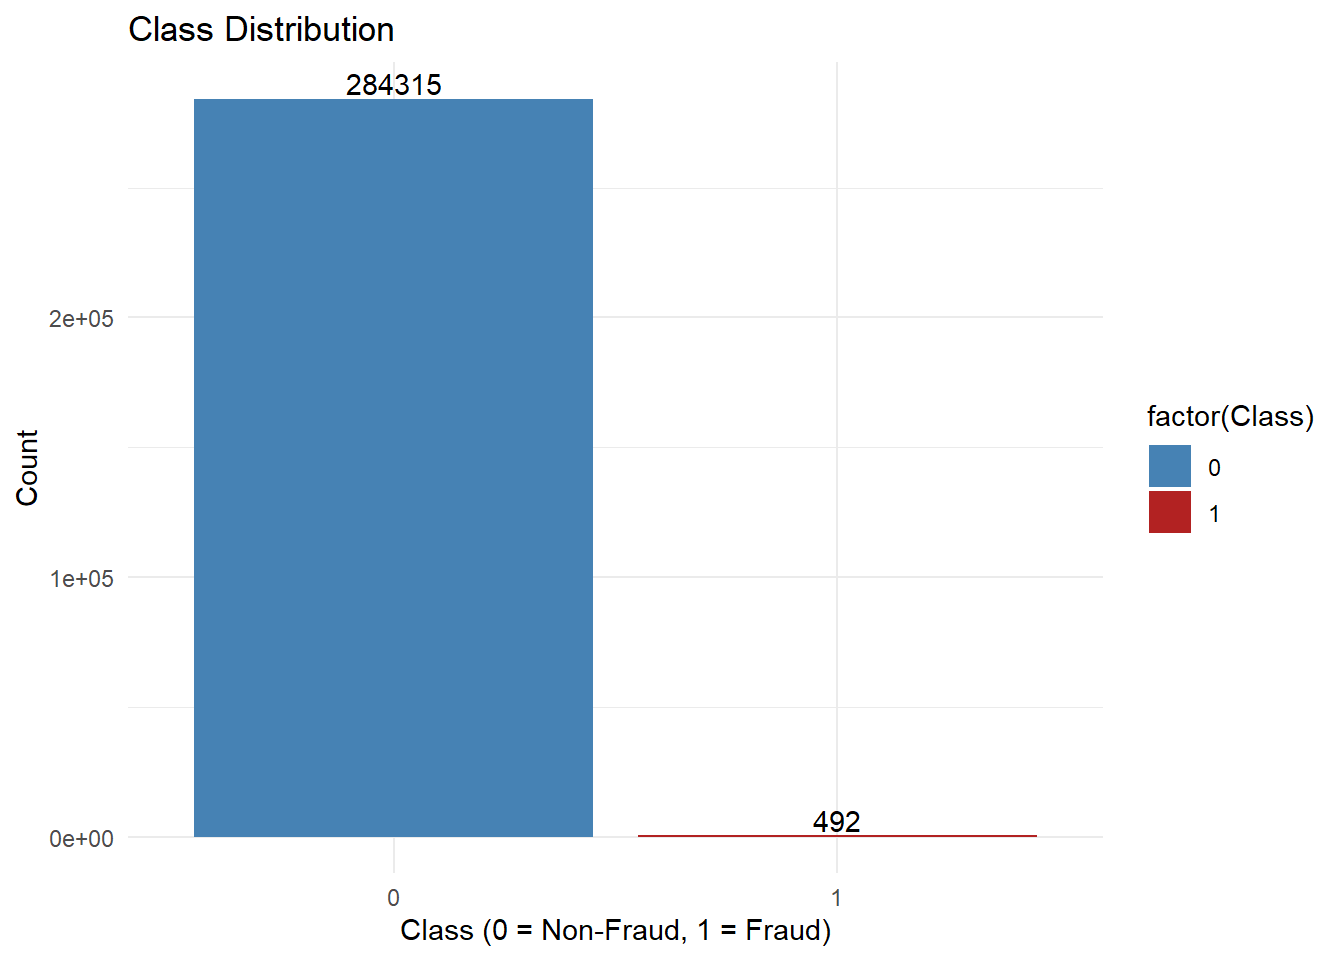
\includegraphics{final_report1_files/figure-pdf/unnamed-chunk-3-1.pdf}

This bar chart shows the number of transactions for each class in our
dataset. We clearly see a massive imbalance:

There are 284,315 non-fraudulent transactions (class 0), making up
nearly 99.83\% of the data.

In contrast, there are only 492 fraudulent transactions (class 1), which
is about 0.17\% of the total.

If we trained a model without addressing this imbalance, it might just
predict ``non-fraud'' for everything and still appear 99.8\%
``accurate'' --- but it would fail to catch real fraud. This makes it
essential to use resampling methods (like SMOTE or ROSE).

2. Visualize Transaction Amount by Class

\begin{Shaded}
\begin{Highlighting}[]
\FunctionTok{ggplot}\NormalTok{(df, }\FunctionTok{aes}\NormalTok{(}\AttributeTok{x =}\NormalTok{ Amount }\SpecialCharTok{+} \DecValTok{1}\NormalTok{, }\AttributeTok{color =} \FunctionTok{factor}\NormalTok{(Class), }\AttributeTok{fill =} \FunctionTok{factor}\NormalTok{(Class))) }\SpecialCharTok{+}
  \FunctionTok{geom\_density}\NormalTok{(}\AttributeTok{alpha =} \FloatTok{0.4}\NormalTok{) }\SpecialCharTok{+}
  \FunctionTok{scale\_x\_log10}\NormalTok{(}\AttributeTok{labels =}\NormalTok{ comma) }\SpecialCharTok{+}
  \FunctionTok{scale\_fill\_manual}\NormalTok{(}\AttributeTok{values =} \FunctionTok{c}\NormalTok{(}\StringTok{"steelblue"}\NormalTok{, }\StringTok{"firebrick"}\NormalTok{), }\AttributeTok{labels =} \FunctionTok{c}\NormalTok{(}\StringTok{"Non{-}Fraud"}\NormalTok{, }\StringTok{"Fraud"}\NormalTok{)) }\SpecialCharTok{+}
  \FunctionTok{scale\_color\_manual}\NormalTok{(}\AttributeTok{values =} \FunctionTok{c}\NormalTok{(}\StringTok{"steelblue"}\NormalTok{, }\StringTok{"firebrick"}\NormalTok{), }\AttributeTok{labels =} \FunctionTok{c}\NormalTok{(}\StringTok{"Non{-}Fraud"}\NormalTok{, }\StringTok{"Fraud"}\NormalTok{)) }\SpecialCharTok{+}
  \FunctionTok{labs}\NormalTok{(}
    \AttributeTok{title =} \StringTok{"Density of Transaction Amount by Class"}\NormalTok{,}
    \AttributeTok{x =} \StringTok{"Transaction Amount (Log Scale)"}\NormalTok{,}
    \AttributeTok{y =} \StringTok{"Density"}\NormalTok{,}
    \AttributeTok{fill =} \StringTok{"Transaction Type"}\NormalTok{,}
    \AttributeTok{color =} \StringTok{"Transaction Type"}
\NormalTok{  ) }\SpecialCharTok{+}
  \FunctionTok{theme\_minimal}\NormalTok{()}
\end{Highlighting}
\end{Shaded}

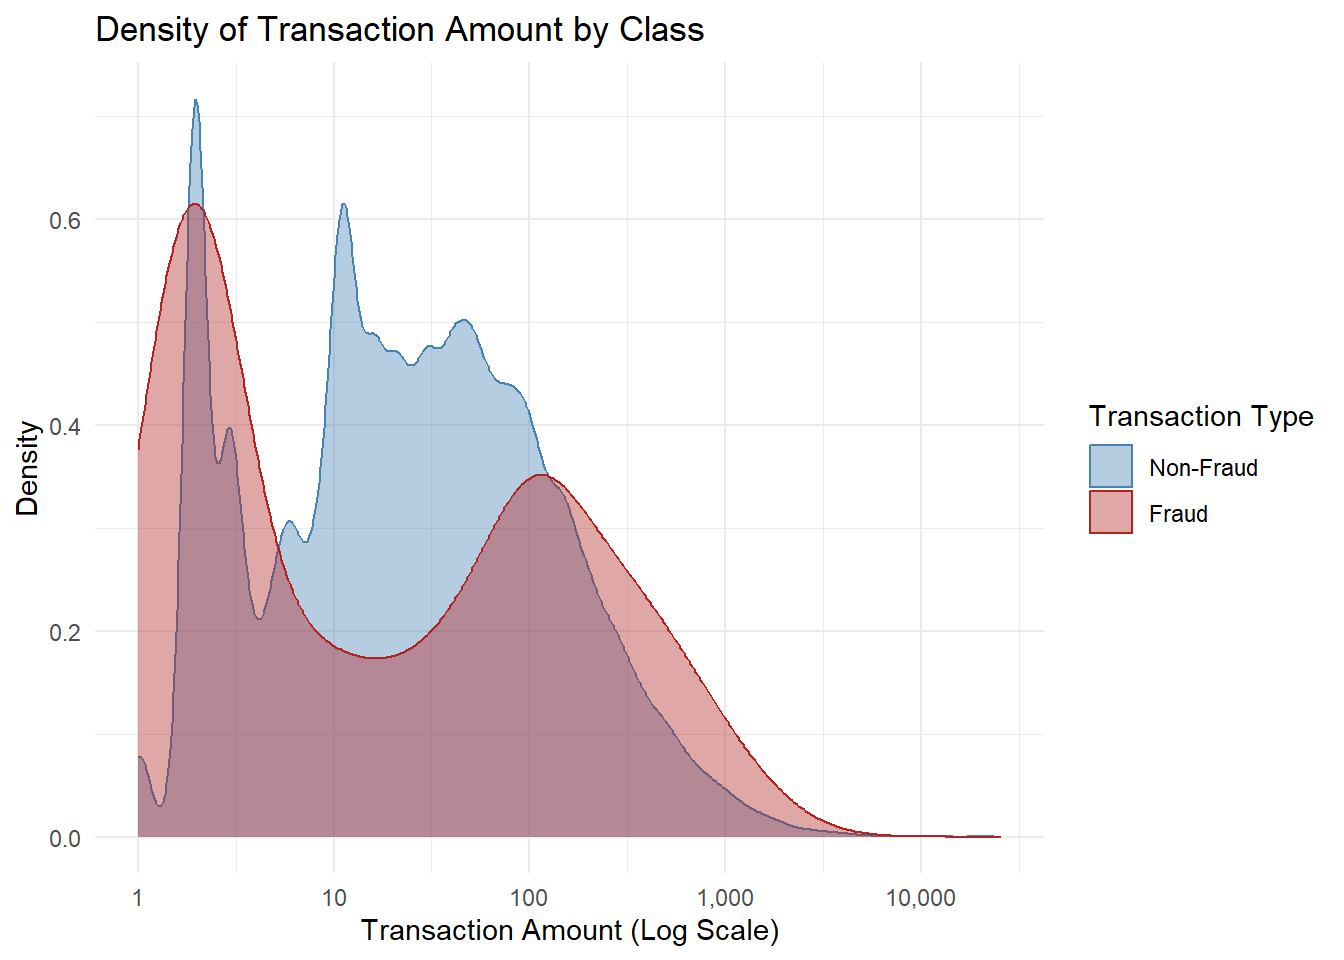
\includegraphics{final_report1_files/figure-pdf/unnamed-chunk-4-1.pdf}

This plot reveals that fraudulent transactions tend to cluster around
lower amounts, while non-fraudulent transactions are spread across a
broader range. Fraud shows higher density below 100 units, hinting at a
preference for small-value fraudulent actions.

\begin{Shaded}
\begin{Highlighting}[]
\FunctionTok{ggplot}\NormalTok{(df, }\FunctionTok{aes}\NormalTok{(}\AttributeTok{x =}\NormalTok{ Amount }\SpecialCharTok{+} \DecValTok{1}\NormalTok{, }\AttributeTok{fill =} \FunctionTok{factor}\NormalTok{(Class))) }\SpecialCharTok{+}
  \FunctionTok{geom\_histogram}\NormalTok{(}\AttributeTok{bins =} \DecValTok{100}\NormalTok{, }\AttributeTok{position =} \StringTok{"identity"}\NormalTok{, }\AttributeTok{alpha =} \FloatTok{0.6}\NormalTok{) }\SpecialCharTok{+}
  \FunctionTok{scale\_x\_log10}\NormalTok{(}\AttributeTok{labels =}\NormalTok{ comma) }\SpecialCharTok{+}
  \FunctionTok{scale\_fill\_manual}\NormalTok{(}\AttributeTok{values =} \FunctionTok{c}\NormalTok{(}\StringTok{"steelblue"}\NormalTok{, }\StringTok{"firebrick"}\NormalTok{), }\AttributeTok{labels =} \FunctionTok{c}\NormalTok{(}\StringTok{"Non{-}Fraud"}\NormalTok{, }\StringTok{"Fraud"}\NormalTok{)) }\SpecialCharTok{+}
  \FunctionTok{labs}\NormalTok{(}
    \AttributeTok{title =} \StringTok{"Transaction Amount by Class"}\NormalTok{,}
    \AttributeTok{x =} \StringTok{"Transaction Amount (Log Scale)"}\NormalTok{,}
    \AttributeTok{y =} \StringTok{"Count"}\NormalTok{,}
    \AttributeTok{fill =} \StringTok{"Transaction Type"}
\NormalTok{  ) }\SpecialCharTok{+}
  \FunctionTok{theme\_minimal}\NormalTok{()}
\end{Highlighting}
\end{Shaded}

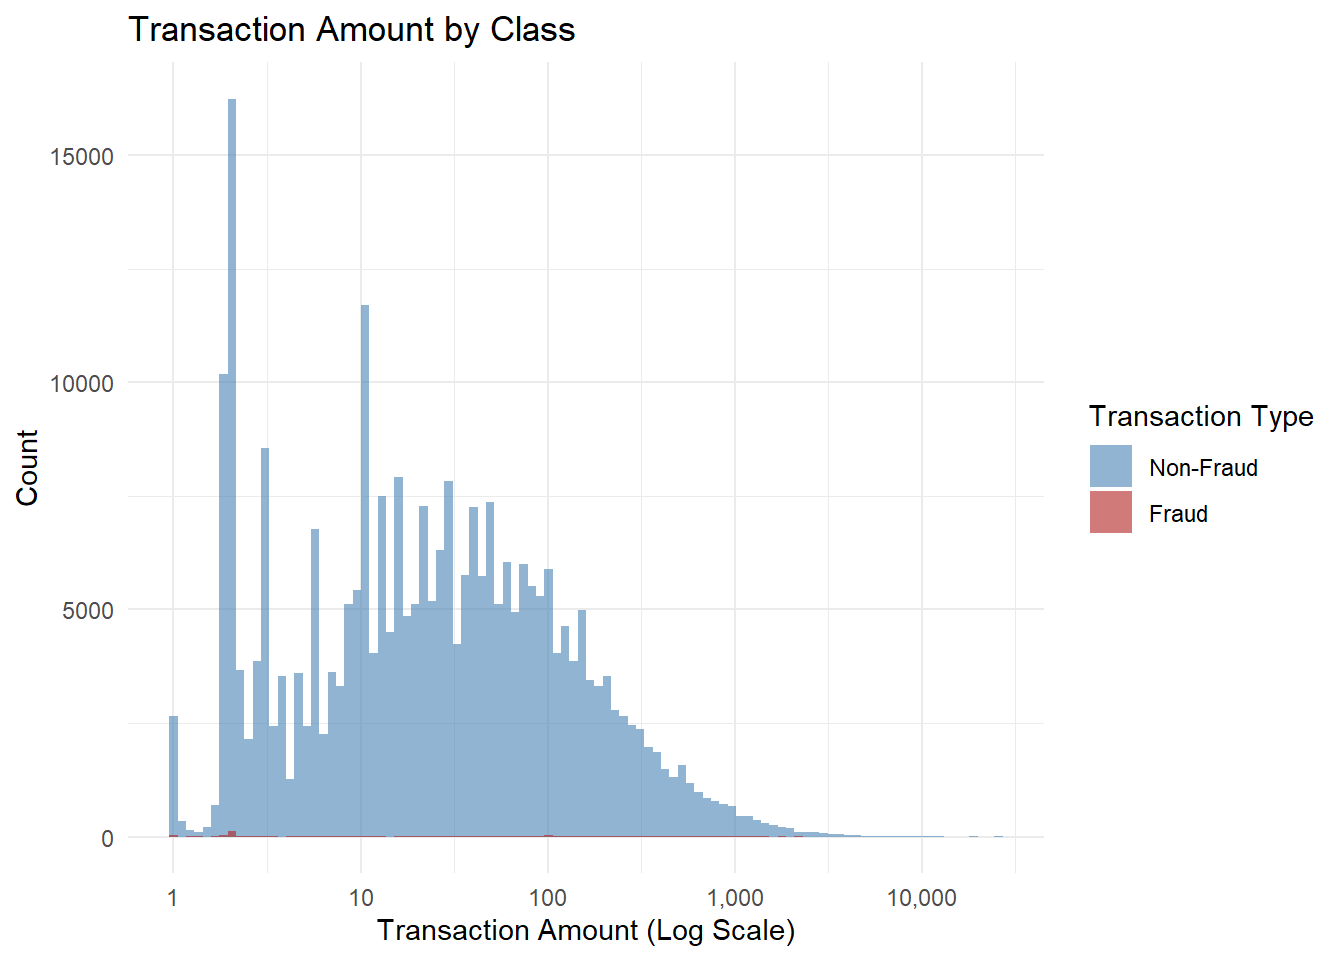
\includegraphics{final_report1_files/figure-pdf/unnamed-chunk-5-1.pdf}

\begin{Shaded}
\begin{Highlighting}[]
\FunctionTok{ggplot}\NormalTok{(df, }\FunctionTok{aes}\NormalTok{(}\AttributeTok{x =} \FunctionTok{factor}\NormalTok{(Class), }\AttributeTok{y =}\NormalTok{ Amount)) }\SpecialCharTok{+}
  \FunctionTok{geom\_boxplot}\NormalTok{() }\SpecialCharTok{+}
  \FunctionTok{labs}\NormalTok{(}\AttributeTok{title =} \StringTok{"Boxplots of Amount by Class"}\NormalTok{,}
       \AttributeTok{x =} \StringTok{"Class"}\NormalTok{,}
       \AttributeTok{y =} \StringTok{"Amount"}\NormalTok{) }\SpecialCharTok{+}
  \FunctionTok{theme\_minimal}\NormalTok{()}
\end{Highlighting}
\end{Shaded}

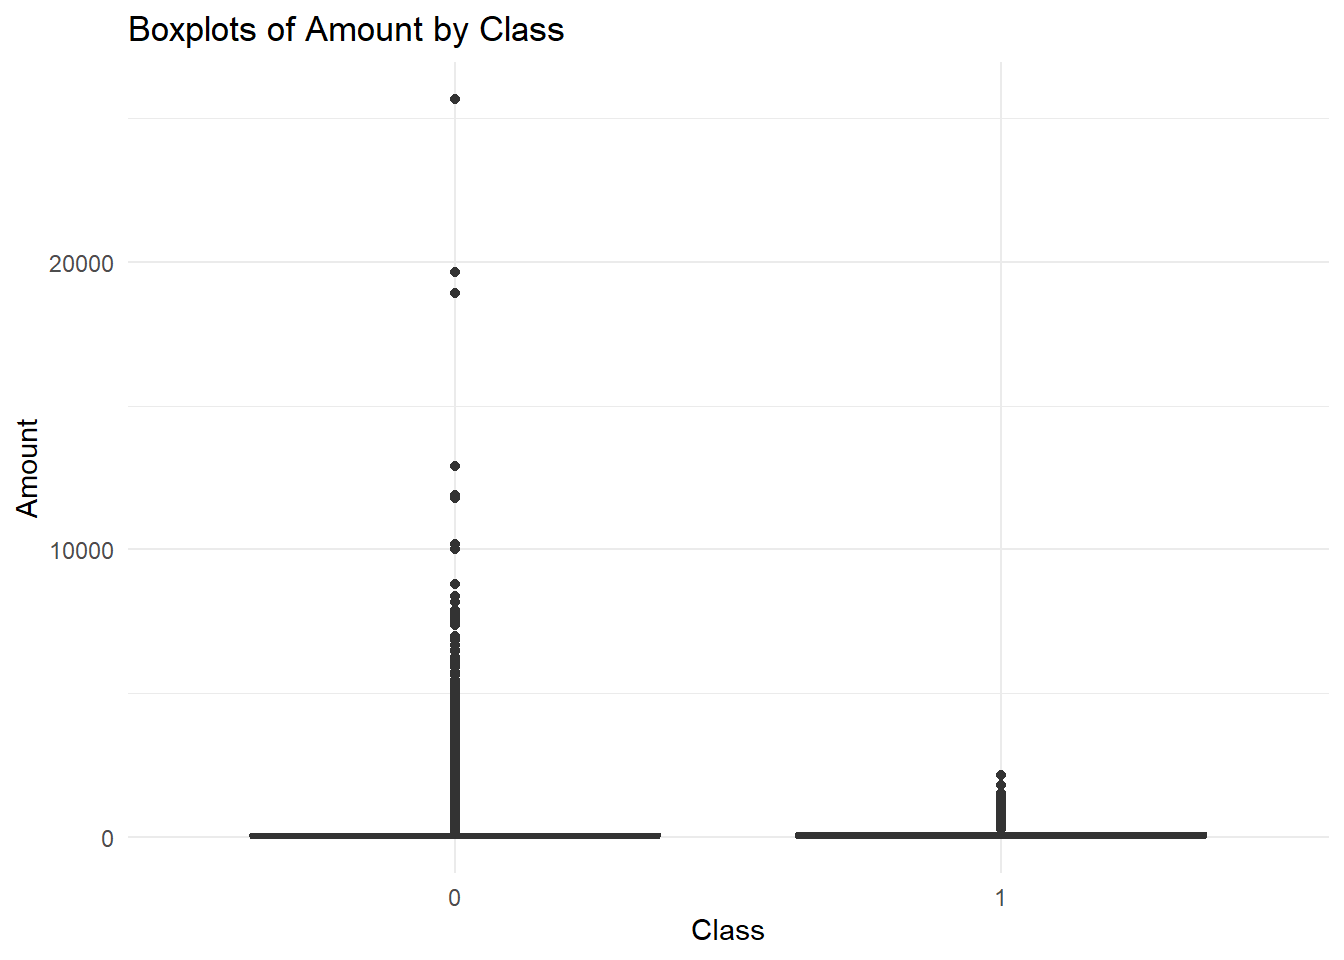
\includegraphics{final_report1_files/figure-pdf/unnamed-chunk-6-1.pdf}

3. Transaction Time by Class

\begin{Shaded}
\begin{Highlighting}[]
\FunctionTok{ggplot}\NormalTok{(df, }\FunctionTok{aes}\NormalTok{(}\AttributeTok{x =}\NormalTok{ Hour, }\AttributeTok{fill =} \FunctionTok{factor}\NormalTok{(Class), }\AttributeTok{color =} \FunctionTok{factor}\NormalTok{(Class))) }\SpecialCharTok{+}
  \FunctionTok{geom\_density}\NormalTok{(}\AttributeTok{alpha =} \FloatTok{0.4}\NormalTok{, }\AttributeTok{adjust =} \FloatTok{1.2}\NormalTok{, }\AttributeTok{bw =} \FloatTok{0.1}\NormalTok{) }\SpecialCharTok{+}
  \FunctionTok{scale\_fill\_manual}\NormalTok{(}\AttributeTok{values =} \FunctionTok{c}\NormalTok{(}\StringTok{"steelblue"}\NormalTok{, }\StringTok{"firebrick"}\NormalTok{), }\AttributeTok{labels =} \FunctionTok{c}\NormalTok{(}\StringTok{"Non{-}Fraud"}\NormalTok{, }\StringTok{"Fraud"}\NormalTok{)) }\SpecialCharTok{+}
  \FunctionTok{scale\_color\_manual}\NormalTok{(}\AttributeTok{values =} \FunctionTok{c}\NormalTok{(}\StringTok{"steelblue"}\NormalTok{, }\StringTok{"firebrick"}\NormalTok{), }\AttributeTok{labels =} \FunctionTok{c}\NormalTok{(}\StringTok{"Non{-}Fraud"}\NormalTok{, }\StringTok{"Fraud"}\NormalTok{)) }\SpecialCharTok{+}
  \FunctionTok{labs}\NormalTok{(}
    \AttributeTok{title =} \StringTok{"Density of Transactions by Hour of Day"}\NormalTok{,}
    \AttributeTok{x =} \StringTok{"Hour of Day"}\NormalTok{,}
    \AttributeTok{y =} \StringTok{"Density"}\NormalTok{,}
    \AttributeTok{fill =} \StringTok{"Class"}\NormalTok{,}
    \AttributeTok{color =} \StringTok{"Class"}
\NormalTok{  ) }\SpecialCharTok{+}
  \FunctionTok{theme\_minimal}\NormalTok{()}
\end{Highlighting}
\end{Shaded}

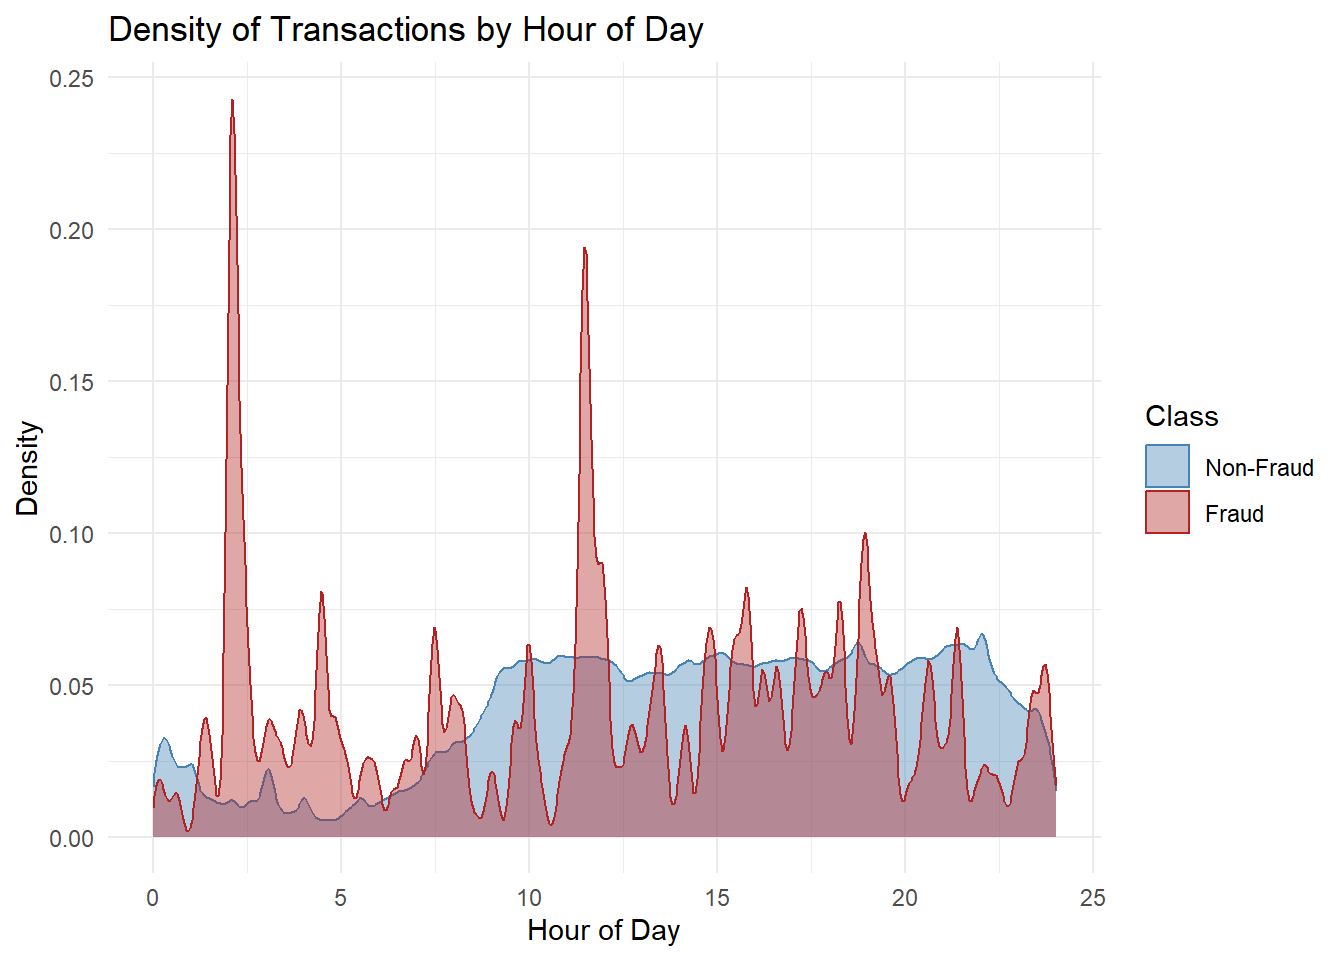
\includegraphics{final_report1_files/figure-pdf/unnamed-chunk-7-1.pdf}

This plot shows when during the day fraudulent vs.~non-fraudulent
transactions are most likely to occur. Although the dataset spans two
days, we compress both days into a 24-hour cycle to capture daily
patterns.

Non-fraudulent transactions are fairly evenly distributed throughout the
day, with a peak during business hours.

Fraudulent transactions, however, appear slightly more concentrated in
the early morning (around 1--6 AM), when regular activity is lower.

This could suggest that fraud attempts are more likely to occur when
users or bank systems are less active, possibly to avoid detection.

\begin{enumerate}
\def\labelenumi{\arabic{enumi}.}
\setcounter{enumi}{3}
\tightlist
\item
  Correlation Matrix of Features
\end{enumerate}

\begin{Shaded}
\begin{Highlighting}[]
\CommentTok{\# Compute correlation matrix}
\NormalTok{cor\_matrix }\OtherTok{\textless{}{-}} \FunctionTok{cor}\NormalTok{(df[, }\SpecialCharTok{{-}}\FunctionTok{which}\NormalTok{(}\FunctionTok{names}\NormalTok{(df) }\SpecialCharTok{==} \StringTok{"Class"}\NormalTok{)])  }\CommentTok{\# Exclude \textquotesingle{}Class\textquotesingle{}}

\CommentTok{\# Base R heatmap using corrplot}
\FunctionTok{corrplot}\NormalTok{(cor\_matrix, }\AttributeTok{method =} \StringTok{"color"}\NormalTok{, }\AttributeTok{type =} \StringTok{"upper"}\NormalTok{, }
         \AttributeTok{tl.cex =} \FloatTok{0.7}\NormalTok{, }\AttributeTok{tl.col =} \StringTok{"black"}\NormalTok{, }\AttributeTok{title =} \StringTok{"Correlation Heatmap"}\NormalTok{, }\AttributeTok{mar =} \FunctionTok{c}\NormalTok{(}\DecValTok{0}\NormalTok{,}\DecValTok{0}\NormalTok{,}\DecValTok{1}\NormalTok{,}\DecValTok{0}\NormalTok{))}
\end{Highlighting}
\end{Shaded}

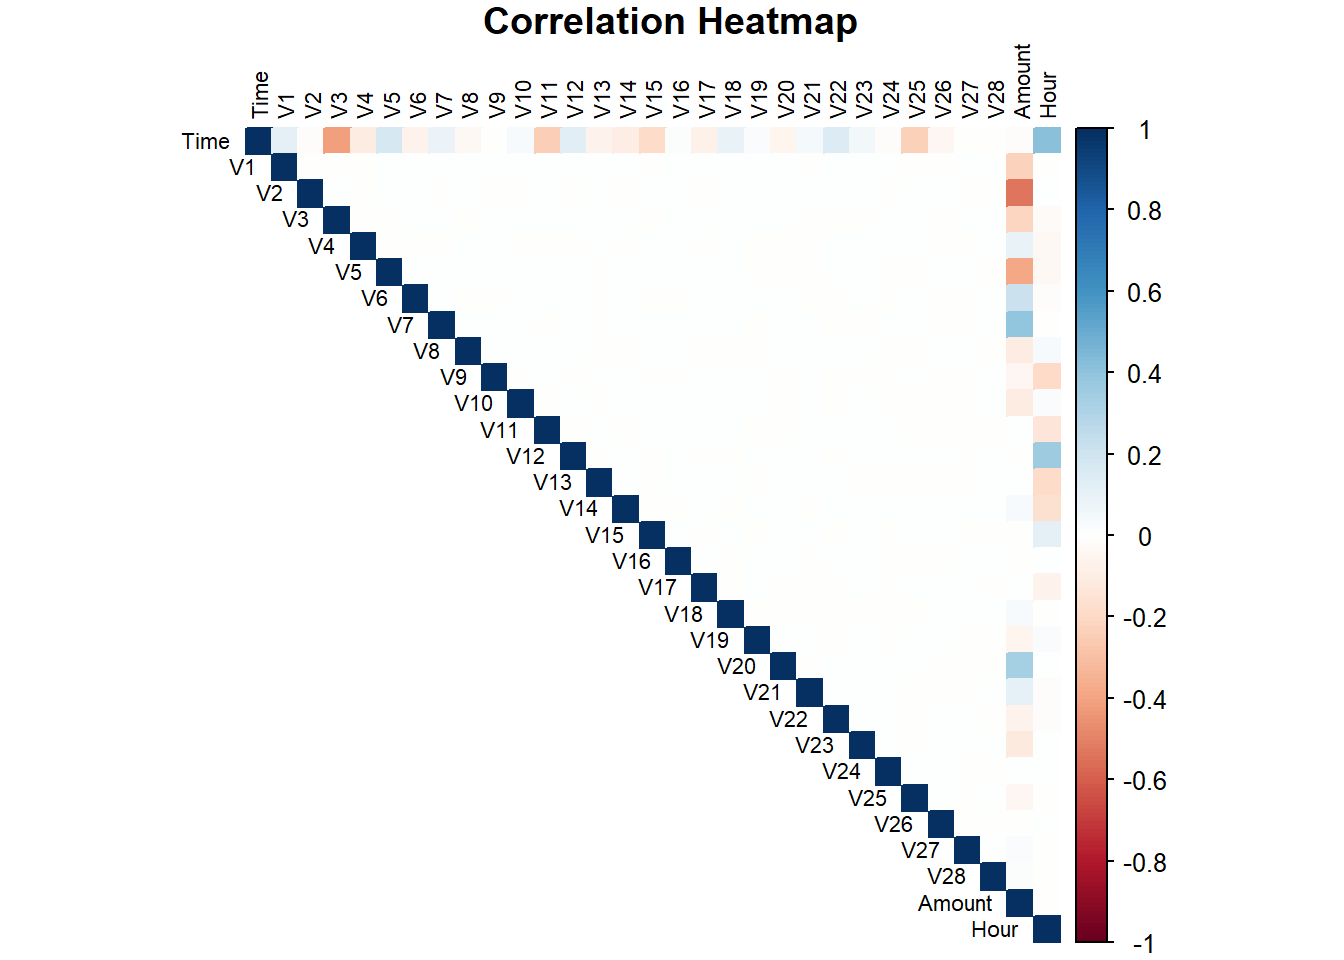
\includegraphics{final_report1_files/figure-pdf/unnamed-chunk-8-1.pdf}

\begin{enumerate}
\def\labelenumi{\arabic{enumi}.}
\setcounter{enumi}{4}
\item
  T-test on Amount for Fraud vs.~Non-Fraud

\begin{Shaded}
\begin{Highlighting}[]
\NormalTok{t\_test\_result }\OtherTok{\textless{}{-}} \FunctionTok{t.test}\NormalTok{(Amount }\SpecialCharTok{\textasciitilde{}}\NormalTok{ Class, }\AttributeTok{data =}\NormalTok{ df)}
\FunctionTok{print}\NormalTok{(t\_test\_result)}
\end{Highlighting}
\end{Shaded}

\begin{verbatim}

    Welch Two Sample t-test

data:  Amount by Class
t = -2.9288, df = 492.61, p-value = 0.003561
alternative hypothesis: true difference in means between group 0 and group 1 is not equal to 0
95 percent confidence interval:
 -56.67588 -11.16472
sample estimates:
mean in group 0 mean in group 1 
       88.29102       122.21132 
\end{verbatim}
\end{enumerate}

\subsection{Resampling}\label{resampling}

\begin{Shaded}
\begin{Highlighting}[]
\CommentTok{\# Check class imbalance}
\FunctionTok{table}\NormalTok{(df}\SpecialCharTok{$}\NormalTok{Class)}
\end{Highlighting}
\end{Shaded}

\begin{verbatim}

     0      1 
284315    492 
\end{verbatim}

\begin{Shaded}
\begin{Highlighting}[]
\FunctionTok{prop.table}\NormalTok{(}\FunctionTok{table}\NormalTok{(df}\SpecialCharTok{$}\NormalTok{Class))  }\CommentTok{\# Percent fraud vs. normal}
\end{Highlighting}
\end{Shaded}

\begin{verbatim}

          0           1 
0.998272514 0.001727486 
\end{verbatim}

We'll keep all the fraud cases (Class = 1), generate synthetic ones, and
reduce the number of non-fraud cases (Class = 0) to create a balanced
training set.

\begin{Shaded}
\begin{Highlighting}[]
\NormalTok{df}\SpecialCharTok{$}\NormalTok{Class }\OtherTok{\textless{}{-}} \FunctionTok{as.factor}\NormalTok{(df}\SpecialCharTok{$}\NormalTok{Class)}
\end{Highlighting}
\end{Shaded}

\begin{Shaded}
\begin{Highlighting}[]
\CommentTok{\# Apply SMOTE with Undersampling}
\FunctionTok{set.seed}\NormalTok{(}\DecValTok{1}\NormalTok{)}

\NormalTok{df\_smote\_under }\OtherTok{\textless{}{-}} \FunctionTok{SMOTE}\NormalTok{(Class }\SpecialCharTok{\textasciitilde{}}\NormalTok{ ., }\AttributeTok{data =}\NormalTok{ df, }\AttributeTok{perc.over =} \DecValTok{600}\NormalTok{, }\AttributeTok{perc.under =} \DecValTok{100}\NormalTok{)}

\FunctionTok{table}\NormalTok{(df\_smote\_under}\SpecialCharTok{$}\NormalTok{Class)}
\end{Highlighting}
\end{Shaded}

\begin{verbatim}

   0    1 
2952 3444 
\end{verbatim}

perc.over = 600 → SMOTE created 6 synthetic cases per real fraud → 492 ×
6 = 2952 synthetic frauds

Total frauds after SMOTE = 492 original + 2952 synthetic = 3444

perc.under = 100 → You keep 1 non-fraud for each fraud → So, 2952
non-frauds were selected from the original 284,315

\begin{Shaded}
\begin{Highlighting}[]
\FunctionTok{ggplot}\NormalTok{(df\_smote\_under, }\FunctionTok{aes}\NormalTok{(}\AttributeTok{x =}\NormalTok{ Class)) }\SpecialCharTok{+}
  \FunctionTok{geom\_bar}\NormalTok{(}\AttributeTok{fill =} \FunctionTok{c}\NormalTok{(}\StringTok{"steelblue"}\NormalTok{, }\StringTok{"firebrick"}\NormalTok{)) }\SpecialCharTok{+}
  \FunctionTok{labs}\NormalTok{(}\AttributeTok{title =} \StringTok{"Class Distribution After SMOTE + Undersampling"}\NormalTok{, }\AttributeTok{x =} \StringTok{"Class"}\NormalTok{, }\AttributeTok{y =} \StringTok{"Count"}\NormalTok{) }\SpecialCharTok{+}
  \FunctionTok{theme\_minimal}\NormalTok{()}
\end{Highlighting}
\end{Shaded}

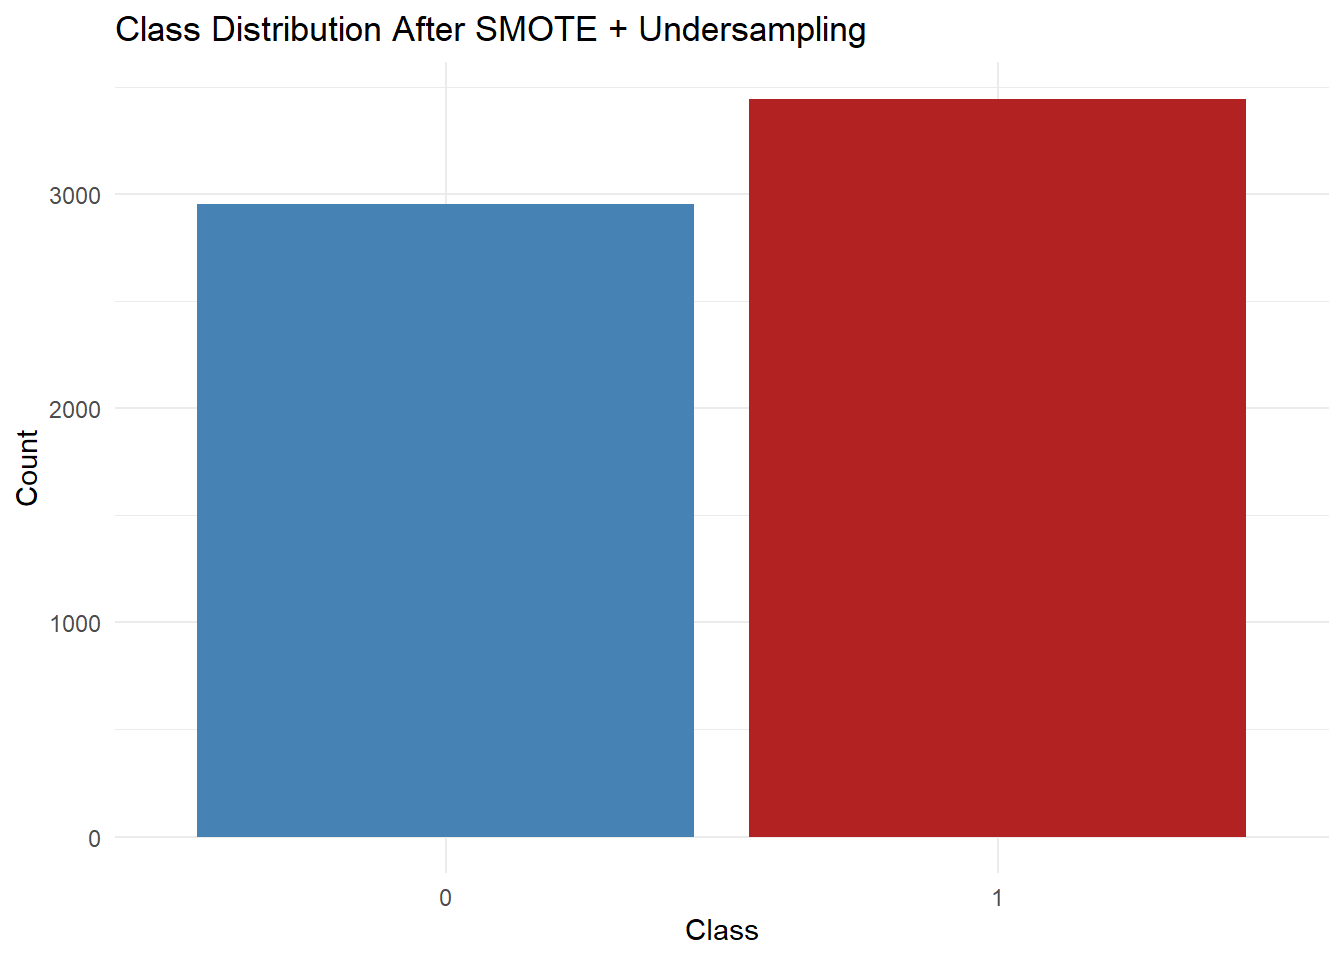
\includegraphics{final_report1_files/figure-pdf/unnamed-chunk-13-1.pdf}

After applying SMOTE with 600\% oversampling and 1:1 undersampling, we
generated 3444 fraud cases (492 real + 2952 synthetic) and kept 2952
non-fraud cases. This gives us a nearly balanced dataset (54\% fraud
vs.~46\% non-fraud) suitable for training without being overwhelmed by
majority class bias.

\subsection{Basic Model Fitting with Original Data
Set}\label{basic-model-fitting-with-original-data-set}

\begin{enumerate}
\def\labelenumi{\arabic{enumi}.}
\item
  Scale the Features

\begin{Shaded}
\begin{Highlighting}[]
\NormalTok{features }\OtherTok{\textless{}{-}}\NormalTok{ df[, }\FunctionTok{setdiff}\NormalTok{(}\FunctionTok{names}\NormalTok{(df), }\StringTok{"Class"}\NormalTok{)]}

\CommentTok{\# Scale features}
\NormalTok{scaled\_features }\OtherTok{\textless{}{-}} \FunctionTok{as.data.frame}\NormalTok{(}\FunctionTok{scale}\NormalTok{(features))}

\CommentTok{\# Combine with target column}
\NormalTok{df\_scaled }\OtherTok{\textless{}{-}} \FunctionTok{cbind}\NormalTok{(scaled\_features, }\AttributeTok{Class =}\NormalTok{ df}\SpecialCharTok{$}\NormalTok{Class)}
\end{Highlighting}
\end{Shaded}
\item
  Create Train/Test Split

\begin{Shaded}
\begin{Highlighting}[]
\FunctionTok{set.seed}\NormalTok{(}\DecValTok{123}\NormalTok{)}
\NormalTok{df\_scaled}\SpecialCharTok{$}\NormalTok{Class }\OtherTok{\textless{}{-}} \FunctionTok{as.factor}\NormalTok{(df\_scaled}\SpecialCharTok{$}\NormalTok{Class)}
\NormalTok{train\_index }\OtherTok{\textless{}{-}} \FunctionTok{createDataPartition}\NormalTok{(df\_scaled}\SpecialCharTok{$}\NormalTok{Class, }\AttributeTok{p =} \FloatTok{0.7}\NormalTok{, }\AttributeTok{list =} \ConstantTok{FALSE}\NormalTok{)}

\NormalTok{train\_data }\OtherTok{\textless{}{-}}\NormalTok{ df\_scaled[train\_index, ]}
\NormalTok{test\_data  }\OtherTok{\textless{}{-}}\NormalTok{ df\_scaled[}\SpecialCharTok{{-}}\NormalTok{train\_index, ]}
\end{Highlighting}
\end{Shaded}
\item
  Fit a Logistic Regression Model using whole data

\begin{Shaded}
\begin{Highlighting}[]
\CommentTok{\# Fit initial logistic model on all predictors}
\NormalTok{initial\_model }\OtherTok{\textless{}{-}} \FunctionTok{glm}\NormalTok{(Class }\SpecialCharTok{\textasciitilde{}}\NormalTok{ ., }\AttributeTok{data =}\NormalTok{ train\_data, }\AttributeTok{family =}\NormalTok{ binomial)}

\FunctionTok{summary}\NormalTok{(initial\_model)}
\end{Highlighting}
\end{Shaded}

\begin{verbatim}

Call:
glm(formula = Class ~ ., family = binomial, data = train_data)

Coefficients:
            Estimate Std. Error z value Pr(>|z|)    
(Intercept) -8.75739    0.18354 -47.715  < 2e-16 ***
V1           0.20826    0.10623   1.960 0.049949 *  
V2           0.02583    0.11885   0.217 0.827943    
V3           0.08172    0.08769   0.932 0.351361    
V4           1.03880    0.13335   7.790 6.71e-15 ***
V5           0.16737    0.11071   1.512 0.130566    
V6          -0.10918    0.12198  -0.895 0.370747    
V7          -0.15976    0.10538  -1.516 0.129498    
V8          -0.21197    0.04763  -4.451 8.57e-06 ***
V9          -0.23356    0.15428  -1.514 0.130069    
V10         -0.98031    0.13784  -7.112 1.14e-12 ***
V11          0.12477    0.09806   1.272 0.203212    
V12         -0.05018    0.11509  -0.436 0.662815    
V13         -0.18810    0.10259  -1.833 0.066738 .  
V14         -0.46986    0.07399  -6.350 2.15e-10 ***
V15         -0.14419    0.09721  -1.483 0.138017    
V16         -0.20490    0.13518  -1.516 0.129565    
V17         -0.01208    0.07458  -0.162 0.871283    
V18         -0.01229    0.13267  -0.093 0.926180    
V19          0.02439    0.09881   0.247 0.805006    
V20         -0.36865    0.08875  -4.154 3.27e-05 ***
V21          0.20600    0.05594   3.683 0.000231 ***
V22          0.29387    0.11593   2.535 0.011250 *  
V23         -0.05825    0.04267  -1.365 0.172191    
V24          0.09914    0.11312   0.876 0.380804    
V25         -0.05208    0.08487  -0.614 0.539512    
V26         -0.15603    0.12010  -1.299 0.193882    
V27         -0.30696    0.07084  -4.333 1.47e-05 ***
V28         -0.08484    0.03757  -2.258 0.023941 *  
Amount       0.21982    0.11568   1.900 0.057401 .  
Hour         0.11945    0.11962   0.999 0.317999    
---
Signif. codes:  0 '***' 0.001 '**' 0.01 '*' 0.05 '.' 0.1 ' ' 1

(Dispersion parameter for binomial family taken to be 1)

    Null deviance: 5077.4  on 199365  degrees of freedom
Residual deviance: 1403.3  on 199335  degrees of freedom
AIC: 1465.3

Number of Fisher Scoring iterations: 12
\end{verbatim}
\item
  Check Variance Inflation Factor for Multicollinearity

\begin{Shaded}
\begin{Highlighting}[]
\FunctionTok{vif}\NormalTok{(initial\_model)}
\end{Highlighting}
\end{Shaded}

\begin{verbatim}
       V1        V2        V3        V4        V5        V6        V7        V8 
 7.280154 13.952606  5.258596  4.322648  8.255510  3.841172  9.450485  2.396360 
       V9       V10       V11       V12       V13       V14       V15       V16 
 5.380269  8.718316  2.552058  6.447101  1.240800  4.992102  1.336216  9.008872 
      V17       V18       V19       V20       V21       V22       V23       V24 
 8.834502  6.644131  2.399256  9.621105  2.577871  3.231270  2.610319  1.464988 
      V25       V26       V27       V28    Amount      Hour 
 1.995120  1.431975  6.821556  1.962003 20.757140  1.527513 
\end{verbatim}
\end{enumerate}

Rule of thumb --\textgreater{} Vif \textgreater10 is a sign of
multicollinearity --\textgreater{} we have many values \textgreater10

\begin{Shaded}
\begin{Highlighting}[]
\NormalTok{log\_prob }\OtherTok{\textless{}{-}} \FunctionTok{predict}\NormalTok{(initial\_model, }\AttributeTok{newdata =}\NormalTok{ test\_data, }\AttributeTok{type =} \StringTok{"response"}\NormalTok{)}
\end{Highlighting}
\end{Shaded}

\subsection{Model with Regularization
(LASSO)}\label{model-with-regularization-lasso}

\begin{Shaded}
\begin{Highlighting}[]
\FunctionTok{h2o.init}\NormalTok{(}\AttributeTok{nthreads =} \SpecialCharTok{{-}}\DecValTok{1}\NormalTok{)}
\end{Highlighting}
\end{Shaded}

\begin{verbatim}
 Connection successful!

R is connected to the H2O cluster: 
    H2O cluster uptime:         7 minutes 304 milliseconds 
    H2O cluster timezone:       Europe/Vienna 
    H2O data parsing timezone:  UTC 
    H2O cluster version:        3.44.0.3 
    H2O cluster version age:    1 year, 6 months and 4 days 
    H2O cluster name:           H2O_started_from_R_sarp_afb950 
    H2O cluster total nodes:    1 
    H2O cluster total memory:   7.69 GB 
    H2O cluster total cores:    20 
    H2O cluster allowed cores:  20 
    H2O cluster healthy:        TRUE 
    H2O Connection ip:          localhost 
    H2O Connection port:        54321 
    H2O Connection proxy:       NA 
    H2O Internal Security:      FALSE 
    R Version:                  R version 4.4.1 (2024-06-14 ucrt) 
\end{verbatim}

\begin{verbatim}
Warning in h2o.clusterInfo(): 
Your H2O cluster version is (1 year, 6 months and 4 days) old. There may be a newer version available.
Please download and install the latest version from: https://h2o-release.s3.amazonaws.com/h2o/latest_stable.html
\end{verbatim}

\begin{Shaded}
\begin{Highlighting}[]
\CommentTok{\# Convert to H2O frame}
\NormalTok{train\_h2o }\OtherTok{\textless{}{-}} \FunctionTok{as.h2o}\NormalTok{(train\_data)}
\end{Highlighting}
\end{Shaded}

\begin{verbatim}

  |                                                                            
  |                                                                      |   0%
  |                                                                            
  |======================================================================| 100%
\end{verbatim}

\begin{Shaded}
\begin{Highlighting}[]
\NormalTok{test\_h2o }\OtherTok{\textless{}{-}} \FunctionTok{as.h2o}\NormalTok{(test\_data)}
\end{Highlighting}
\end{Shaded}

\begin{verbatim}

  |                                                                            
  |                                                                      |   0%
  |                                                                            
  |======================================================================| 100%
\end{verbatim}

\begin{Shaded}
\begin{Highlighting}[]
\CommentTok{\# Train lasso (lambda search enabled)}
\NormalTok{model }\OtherTok{\textless{}{-}} \FunctionTok{h2o.glm}\NormalTok{(}\AttributeTok{x =} \FunctionTok{setdiff}\NormalTok{(}\FunctionTok{names}\NormalTok{(train\_data), }\StringTok{"Class"}\NormalTok{),}
                 \AttributeTok{y =} \StringTok{"Class"}\NormalTok{,}
                 \AttributeTok{training\_frame =}\NormalTok{ train\_h2o,}
                 \AttributeTok{family =} \StringTok{"binomial"}\NormalTok{,}
                 \AttributeTok{alpha =} \DecValTok{1}\NormalTok{,}
                 \AttributeTok{lambda\_search =} \ConstantTok{TRUE}\NormalTok{)}
\end{Highlighting}
\end{Shaded}

\begin{verbatim}

  |                                                                            
  |                                                                      |   0%
  |                                                                            
  |======================================================                |  77%
  |                                                                            
  |======================================================================| 100%
\end{verbatim}

\begin{Shaded}
\begin{Highlighting}[]
\CommentTok{\# Predict}
\NormalTok{lasso\_pred }\OtherTok{\textless{}{-}} \FunctionTok{h2o.predict}\NormalTok{(model, test\_h2o)}
\end{Highlighting}
\end{Shaded}

\begin{verbatim}

  |                                                                            
  |                                                                      |   0%
  |                                                                            
  |======================================================================| 100%
\end{verbatim}

\begin{Shaded}
\begin{Highlighting}[]
\NormalTok{lasso\_perf }\OtherTok{\textless{}{-}} \FunctionTok{h2o.performance}\NormalTok{(model, }\AttributeTok{newdata =}\NormalTok{ test\_h2o)}

\CommentTok{\# Plot ROC curve}
\FunctionTok{plot}\NormalTok{(lasso\_perf, }\AttributeTok{type =} \StringTok{"roc"}\NormalTok{)}
\end{Highlighting}
\end{Shaded}

\includegraphics{final_report1_files/figure-pdf/unnamed-chunk-20-1.pdf}

\subsection{Autoencoders for Anomaly
Detection}\label{autoencoders-for-anomaly-detection}

\begin{enumerate}
\def\labelenumi{\arabic{enumi}.}
\tightlist
\item
  Apply autoencoder model
\end{enumerate}

\begin{Shaded}
\begin{Highlighting}[]
\NormalTok{autoencoder }\OtherTok{\textless{}{-}} \FunctionTok{h2o.deeplearning}\NormalTok{(}
  \AttributeTok{x =} \FunctionTok{names}\NormalTok{(scaled\_features),}
  \AttributeTok{training\_frame =}\NormalTok{ train\_h2o,}
  \AttributeTok{autoencoder =} \ConstantTok{TRUE}\NormalTok{,}
  \AttributeTok{hidden =} \FunctionTok{c}\NormalTok{(}\DecValTok{10}\NormalTok{, }\DecValTok{2}\NormalTok{, }\DecValTok{10}\NormalTok{),  }\CommentTok{\# symmetrical bottleneck}
  \AttributeTok{epochs =} \DecValTok{50}\NormalTok{,}
  \AttributeTok{activation =} \StringTok{"Tanh"}\NormalTok{,}
  \AttributeTok{seed =} \DecValTok{123}
\NormalTok{)}
\end{Highlighting}
\end{Shaded}

\begin{verbatim}

  |                                                                            
  |                                                                      |   0%
  |                                                                            
  |====                                                                  |   6%
  |                                                                            
  |===========                                                           |  16%
  |                                                                            
  |===================                                                   |  27%
  |                                                                            
  |==========================                                            |  37%
  |                                                                            
  |==================================                                    |  48%
  |                                                                            
  |=========================================                             |  59%
  |                                                                            
  |================================================                      |  69%
  |                                                                            
  |========================================================              |  80%
  |                                                                            
  |===============================================================       |  90%
  |                                                                            
  |======================================================================| 100%
\end{verbatim}

The small hidden layer (2 in the center) forces the model to compress
information --- anomalies will reconstruct poorly.

\begin{enumerate}
\def\labelenumi{\arabic{enumi}.}
\setcounter{enumi}{2}
\tightlist
\item
  Get Reconstruction Error (Anomaly Score)
\end{enumerate}

\begin{Shaded}
\begin{Highlighting}[]
\NormalTok{recon\_error }\OtherTok{\textless{}{-}} \FunctionTok{h2o.anomaly}\NormalTok{(autoencoder, train\_h2o, }\AttributeTok{per\_feature =} \ConstantTok{FALSE}\NormalTok{)}
\NormalTok{recon\_error\_df }\OtherTok{\textless{}{-}} \FunctionTok{as.data.frame}\NormalTok{(recon\_error)}
\FunctionTok{colnames}\NormalTok{(recon\_error\_df) }\OtherTok{\textless{}{-}} \StringTok{"MSE"}
\end{Highlighting}
\end{Shaded}

\begin{enumerate}
\def\labelenumi{\arabic{enumi}.}
\setcounter{enumi}{3}
\item
  Add Class Labels Back for Evaluation

\begin{Shaded}
\begin{Highlighting}[]
\NormalTok{recon\_error\_df}\SpecialCharTok{$}\NormalTok{Class }\OtherTok{\textless{}{-}}\NormalTok{ train\_data}\SpecialCharTok{$}\NormalTok{Class}
\end{Highlighting}
\end{Shaded}
\item
  Confusion Matrix

\begin{Shaded}
\begin{Highlighting}[]
\NormalTok{threshold }\OtherTok{\textless{}{-}} \FunctionTok{quantile}\NormalTok{(recon\_error\_df}\SpecialCharTok{$}\NormalTok{MSE, }\FloatTok{0.98}\NormalTok{)}

\CommentTok{\# Predict anomalies}
\NormalTok{recon\_error\_df}\SpecialCharTok{$}\NormalTok{pred }\OtherTok{\textless{}{-}} \FunctionTok{ifelse}\NormalTok{(recon\_error\_df}\SpecialCharTok{$}\NormalTok{MSE }\SpecialCharTok{\textgreater{}}\NormalTok{ threshold, }\DecValTok{1}\NormalTok{, }\DecValTok{0}\NormalTok{)}

\FunctionTok{confusionMatrix}\NormalTok{(}\FunctionTok{factor}\NormalTok{(recon\_error\_df}\SpecialCharTok{$}\NormalTok{pred), }\FunctionTok{factor}\NormalTok{(recon\_error\_df}\SpecialCharTok{$}\NormalTok{Class), }\AttributeTok{positive =} \StringTok{"1"}\NormalTok{)}
\end{Highlighting}
\end{Shaded}

\begin{verbatim}
Confusion Matrix and Statistics

          Reference
Prediction      0      1
         0 195286     92
         1   3735    253

               Accuracy : 0.9808          
                 95% CI : (0.9802, 0.9814)
    No Information Rate : 0.9983          
    P-Value [Acc > NIR] : 1               

                  Kappa : 0.114           

 Mcnemar's Test P-Value : <2e-16          

            Sensitivity : 0.733333        
            Specificity : 0.981233        
         Pos Pred Value : 0.063440        
         Neg Pred Value : 0.999529        
             Prevalence : 0.001730        
         Detection Rate : 0.001269        
   Detection Prevalence : 0.020003        
      Balanced Accuracy : 0.857283        

       'Positive' Class : 1               
\end{verbatim}
\item
  Plot the reconstruction error

\begin{Shaded}
\begin{Highlighting}[]
\FunctionTok{ggplot}\NormalTok{(recon\_error\_df, }\FunctionTok{aes}\NormalTok{(}\AttributeTok{x =}\NormalTok{ MSE, }\AttributeTok{fill =} \FunctionTok{factor}\NormalTok{(Class))) }\SpecialCharTok{+}
  \FunctionTok{geom\_density}\NormalTok{(}\AttributeTok{alpha =} \FloatTok{0.5}\NormalTok{) }\SpecialCharTok{+}
  \FunctionTok{labs}\NormalTok{(}\AttributeTok{title =} \StringTok{"Reconstruction Error by Class"}\NormalTok{, }\AttributeTok{x =} \StringTok{"Reconstruction MSE"}\NormalTok{, }\AttributeTok{fill =} \StringTok{"Class"}\NormalTok{) }\SpecialCharTok{+}
  \FunctionTok{theme\_minimal}\NormalTok{()}
\end{Highlighting}
\end{Shaded}

  \includegraphics{final_report1_files/figure-pdf/unnamed-chunk-25-1.pdf}
\end{enumerate}

\subsection{XGBoost Model Original
Data}\label{xgboost-model-original-data}

We proceeded with applying the XGBoost- Extreme Gradient Boosting
algorithm to the data. Given the highly imbalanced credit card fraud
dataset, we aim to inspect the algorithms ability to capture complex
interactions and decision boundaries.

\begin{enumerate}
\def\labelenumi{\arabic{enumi}.}
\tightlist
\item
  Convert data to DMatrix
\end{enumerate}

\begin{Shaded}
\begin{Highlighting}[]
\NormalTok{y\_train\_bin }\OtherTok{\textless{}{-}} \FunctionTok{as.numeric}\NormalTok{(train\_data}\SpecialCharTok{$}\NormalTok{Class) }\SpecialCharTok{{-}} \DecValTok{1}  \CommentTok{\# 1 for "pos", 0 for "neg"}
\NormalTok{y\_test\_bin  }\OtherTok{\textless{}{-}} \FunctionTok{as.numeric}\NormalTok{(test\_data}\SpecialCharTok{$}\NormalTok{Class) }\SpecialCharTok{{-}} \DecValTok{1}

\NormalTok{dtrain }\OtherTok{\textless{}{-}} \FunctionTok{xgb.DMatrix}\NormalTok{(}
  \AttributeTok{data  =} \FunctionTok{as.matrix}\NormalTok{(train\_data[ , }\FunctionTok{setdiff}\NormalTok{(}\FunctionTok{names}\NormalTok{(train\_data), }\StringTok{"Class"}\NormalTok{)]),}
  \AttributeTok{label =}\NormalTok{ y\_train\_bin}
\NormalTok{)}
\NormalTok{dtest }\OtherTok{\textless{}{-}} \FunctionTok{xgb.DMatrix}\NormalTok{(}
  \AttributeTok{data  =} \FunctionTok{as.matrix}\NormalTok{(test\_data[  , }\FunctionTok{setdiff}\NormalTok{(}\FunctionTok{names}\NormalTok{(test\_data),  }\StringTok{"Class"}\NormalTok{)]),}
  \AttributeTok{label =}\NormalTok{ y\_test\_bin}
\NormalTok{)}
\end{Highlighting}
\end{Shaded}

Both test and training data was converted into a special format
xgb.DMatrix. Reasoning:

\begin{itemize}
\item
  optimized for speed and memory efficiency
\item
  supports the weighting of individual rows, which can be used to manage
  class imbalance
\end{itemize}

\begin{enumerate}
\def\labelenumi{\arabic{enumi}.}
\setcounter{enumi}{1}
\tightlist
\item
  Define Hyperparamters
\end{enumerate}

\begin{Shaded}
\begin{Highlighting}[]
\NormalTok{params }\OtherTok{\textless{}{-}} \FunctionTok{list}\NormalTok{(}
  \AttributeTok{objective =} \StringTok{"binary:logistic"}\NormalTok{,}
  \AttributeTok{eval\_metric =} \StringTok{"auc"}\NormalTok{,}
  \AttributeTok{eta =} \FloatTok{0.1}\NormalTok{,}
  \AttributeTok{max\_depth =} \DecValTok{6}
\NormalTok{)}
\end{Highlighting}
\end{Shaded}

The baseline hyperparameters of the XGBoost model are the following

\begin{itemize}
\item
  learning rate of 0.1
\item
  max tree depth of 6 - moderate depth, enough to detect important
  interactions without overly complexity
\item
  early stopping rounds of 10 - stop training if performance on the
  validation set doesn't improve
\item
  auc evaluation metric - wellsuited for imbalanced classification
  problems
\end{itemize}

\begin{enumerate}
\def\labelenumi{\arabic{enumi}.}
\setcounter{enumi}{2}
\tightlist
\item
  Train the Model using df\_scaled training data
\end{enumerate}

\begin{Shaded}
\begin{Highlighting}[]
\NormalTok{xgb\_model }\OtherTok{\textless{}{-}} \FunctionTok{xgb.train}\NormalTok{(}
  \AttributeTok{params =}\NormalTok{ params,}
  \AttributeTok{data =}\NormalTok{ dtrain,}
  \AttributeTok{nrounds =} \DecValTok{100}\NormalTok{,}
  \AttributeTok{watchlist =} \FunctionTok{list}\NormalTok{(}\AttributeTok{train =}\NormalTok{ dtrain, }\AttributeTok{test =}\NormalTok{ dtest),}
  \AttributeTok{early\_stopping\_rounds =} \DecValTok{10}\NormalTok{,}
  \AttributeTok{verbose =} \DecValTok{0}
\NormalTok{)}

\CommentTok{\# Predict probabilities and labels}
\NormalTok{xgb\_pred\_prob }\OtherTok{\textless{}{-}} \FunctionTok{predict}\NormalTok{(xgb\_model, dtest)}
\NormalTok{xgb\_pred\_label }\OtherTok{\textless{}{-}} \FunctionTok{ifelse}\NormalTok{(xgb\_pred\_prob }\SpecialCharTok{\textgreater{}} \FloatTok{0.5}\NormalTok{, }\DecValTok{1}\NormalTok{, }\DecValTok{0}\NormalTok{)}
\end{Highlighting}
\end{Shaded}

The trained XGBoost model generates probabilites on the test set. Hard
class labels are applied to the predicated probability. Within the
thresholds:

\begin{itemize}
\item
  \textgreater{} .50 it is labeled as fraud (1)
\item
  \textless= .50 it is labeled as non-fraud (0)
\end{itemize}

\begin{enumerate}
\def\labelenumi{\arabic{enumi}.}
\setcounter{enumi}{3}
\tightlist
\item
  Inspect Prediction Probability Distribution
\end{enumerate}

\begin{Shaded}
\begin{Highlighting}[]
\FunctionTok{summary}\NormalTok{(xgb\_pred\_prob)}
\end{Highlighting}
\end{Shaded}

\begin{verbatim}
   Min. 1st Qu.  Median    Mean 3rd Qu.    Max. 
 0.1326  0.1326  0.1326  0.1337  0.1326  0.8627 
\end{verbatim}

\begin{Shaded}
\begin{Highlighting}[]
\FunctionTok{hist}\NormalTok{(xgb\_pred\_prob, }\AttributeTok{breaks =} \DecValTok{50}\NormalTok{, }\AttributeTok{main =} \StringTok{"Histogram of Predicted Probabilities"}\NormalTok{, }\AttributeTok{xlab =} \StringTok{"Probability"}\NormalTok{)}
\end{Highlighting}
\end{Shaded}

\includegraphics{final_report1_files/figure-pdf/unnamed-chunk-29-1.pdf}

\begin{enumerate}
\def\labelenumi{\arabic{enumi}.}
\setcounter{enumi}{4}
\tightlist
\item
  Confusion Matrix \& AUC Curve
\end{enumerate}

\begin{Shaded}
\begin{Highlighting}[]
\NormalTok{conf\_matrix }\OtherTok{\textless{}{-}} \FunctionTok{confusionMatrix}\NormalTok{(}
  \FunctionTok{factor}\NormalTok{(xgb\_pred\_label),}
  \FunctionTok{factor}\NormalTok{(}\FunctionTok{getinfo}\NormalTok{(dtest, }\StringTok{"label"}\NormalTok{)),}
  \AttributeTok{positive =} \StringTok{"1"}
\NormalTok{)}
\FunctionTok{print}\NormalTok{(conf\_matrix)}
\end{Highlighting}
\end{Shaded}

\begin{verbatim}
Confusion Matrix and Statistics

          Reference
Prediction     0     1
         0 85285    32
         1     9   115
                                          
               Accuracy : 0.9995          
                 95% CI : (0.9993, 0.9997)
    No Information Rate : 0.9983          
    P-Value [Acc > NIR] : < 2.2e-16       
                                          
                  Kappa : 0.8485          
                                          
 Mcnemar's Test P-Value : 0.0005908       
                                          
            Sensitivity : 0.782313        
            Specificity : 0.999894        
         Pos Pred Value : 0.927419        
         Neg Pred Value : 0.999625        
             Prevalence : 0.001720        
         Detection Rate : 0.001346        
   Detection Prevalence : 0.001451        
      Balanced Accuracy : 0.891104        
                                          
       'Positive' Class : 1               
                                          
\end{verbatim}

\begin{Shaded}
\begin{Highlighting}[]
\CommentTok{\# ROC and AUC}
\NormalTok{roc\_obj }\OtherTok{\textless{}{-}} \FunctionTok{roc}\NormalTok{(}\FunctionTok{getinfo}\NormalTok{(dtest, }\StringTok{"label"}\NormalTok{), xgb\_pred\_prob)}
\end{Highlighting}
\end{Shaded}

\begin{verbatim}
Setting levels: control = 0, case = 1
\end{verbatim}

\begin{verbatim}
Setting direction: controls < cases
\end{verbatim}

\begin{Shaded}
\begin{Highlighting}[]
\FunctionTok{plot}\NormalTok{(roc\_obj, }\AttributeTok{main =} \StringTok{"XGBoost ROC Curve"}\NormalTok{)}
\end{Highlighting}
\end{Shaded}

\includegraphics{final_report1_files/figure-pdf/unnamed-chunk-30-1.pdf}

\begin{Shaded}
\begin{Highlighting}[]
\FunctionTok{cat}\NormalTok{(}\StringTok{"AUC:"}\NormalTok{, }\FunctionTok{auc}\NormalTok{(roc\_obj), }\StringTok{"}\SpecialCharTok{\textbackslash{}n}\StringTok{"}\NormalTok{)}
\end{Highlighting}
\end{Shaded}

\begin{verbatim}
AUC: 0.9113808 
\end{verbatim}

When using the original imbalanced dataset, the ROC curve shows a less
steep shape, and the model is less confident in distinguishing fraud due
to the extreme class imbalance. This limits sensitivity and causes the
ROC curve to underperform. We try to address this with a Resampling
method ROSE.

\subsection{XGBoost with Resampling}\label{xgboost-with-resampling}

Resample the Dataset by oversampling the minority

\begin{enumerate}
\def\labelenumi{\arabic{enumi}.}
\setcounter{enumi}{1}
\tightlist
\item
  Apply ROSE to the scaled data to balance it
\end{enumerate}

\begin{Shaded}
\begin{Highlighting}[]
\FunctionTok{set.seed}\NormalTok{(}\DecValTok{123}\NormalTok{)}
\NormalTok{train\_index }\OtherTok{\textless{}{-}} \FunctionTok{createDataPartition}\NormalTok{(df\_scaled}\SpecialCharTok{$}\NormalTok{Class, }\AttributeTok{p =} \FloatTok{0.7}\NormalTok{, }\AttributeTok{list =} \ConstantTok{FALSE}\NormalTok{)}
\NormalTok{train\_raw }\OtherTok{\textless{}{-}}\NormalTok{ df\_scaled[train\_index, ]}
\NormalTok{test\_data\_xg }\OtherTok{\textless{}{-}}\NormalTok{ df\_scaled[}\SpecialCharTok{{-}}\NormalTok{train\_index, ]}

\CommentTok{\# Now apply ROSE only to the training set}

\NormalTok{train\_data\_xg }\OtherTok{\textless{}{-}} \FunctionTok{ROSE}\NormalTok{(Class }\SpecialCharTok{\textasciitilde{}}\NormalTok{ ., }\AttributeTok{data =}\NormalTok{ train\_raw, }\AttributeTok{seed =} \DecValTok{1}\NormalTok{, }\AttributeTok{N =} \FunctionTok{nrow}\NormalTok{(train\_raw), }\AttributeTok{p =} \FloatTok{0.2}\NormalTok{)}\SpecialCharTok{$}\NormalTok{data}
\end{Highlighting}
\end{Shaded}

\begin{enumerate}
\def\labelenumi{\arabic{enumi}.}
\setcounter{enumi}{3}
\tightlist
\item
  Convert to DMatrix
\end{enumerate}

\begin{Shaded}
\begin{Highlighting}[]
\NormalTok{dtrain\_xg }\OtherTok{\textless{}{-}} \FunctionTok{xgb.DMatrix}\NormalTok{(}
  \AttributeTok{data =} \FunctionTok{as.matrix}\NormalTok{(train\_data\_xg[, }\SpecialCharTok{{-}}\FunctionTok{ncol}\NormalTok{(train\_data\_xg)]), }
  \AttributeTok{label =} \FunctionTok{as.numeric}\NormalTok{(}\FunctionTok{as.character}\NormalTok{(train\_data\_xg}\SpecialCharTok{$}\NormalTok{Class))}
\NormalTok{)}

\NormalTok{dtest\_xg }\OtherTok{\textless{}{-}} \FunctionTok{xgb.DMatrix}\NormalTok{(}
  \AttributeTok{data =} \FunctionTok{as.matrix}\NormalTok{(test\_data\_xg[, }\SpecialCharTok{{-}}\FunctionTok{ncol}\NormalTok{(test\_data\_xg)]), }
  \AttributeTok{label =} \FunctionTok{as.numeric}\NormalTok{(}\FunctionTok{as.character}\NormalTok{(test\_data\_xg}\SpecialCharTok{$}\NormalTok{Class))}
\NormalTok{)}
\end{Highlighting}
\end{Shaded}

\begin{enumerate}
\def\labelenumi{\arabic{enumi}.}
\setcounter{enumi}{4}
\tightlist
\item
  Define Hyperparameters \& create model
\end{enumerate}

\begin{Shaded}
\begin{Highlighting}[]
\NormalTok{params }\OtherTok{\textless{}{-}} \FunctionTok{list}\NormalTok{(}
  \AttributeTok{objective =} \StringTok{"binary:logistic"}\NormalTok{,}
  \AttributeTok{eval\_metric =} \StringTok{"auc"}\NormalTok{,}
  \AttributeTok{eta =} \FloatTok{0.1}\NormalTok{,}
  \AttributeTok{max\_depth =} \DecValTok{6}
\NormalTok{)}

\NormalTok{xgb\_model\_rose }\OtherTok{\textless{}{-}} \FunctionTok{xgb.train}\NormalTok{(}
  \AttributeTok{params =}\NormalTok{ params,}
  \AttributeTok{data =}\NormalTok{ dtrain\_xg,}
  \AttributeTok{nrounds =} \DecValTok{100}\NormalTok{,}
  \AttributeTok{watchlist =} \FunctionTok{list}\NormalTok{(}\AttributeTok{train =}\NormalTok{ dtrain\_xg, }\AttributeTok{test =}\NormalTok{ dtest\_xg),}
  \AttributeTok{early\_stopping\_rounds =} \DecValTok{10}\NormalTok{,}
  \AttributeTok{verbose =} \DecValTok{0}
\NormalTok{)}
\end{Highlighting}
\end{Shaded}

\begin{enumerate}
\def\labelenumi{\arabic{enumi}.}
\setcounter{enumi}{5}
\tightlist
\item
  Predict Probabilities \& Define Threshold
\end{enumerate}

\begin{Shaded}
\begin{Highlighting}[]
\NormalTok{xgb\_rose\_pred\_prob }\OtherTok{\textless{}{-}} \FunctionTok{predict}\NormalTok{(xgb\_model, dtest\_xg)}
\NormalTok{xgb\_rose\_pred\_label }\OtherTok{\textless{}{-}} \FunctionTok{ifelse}\NormalTok{(xgb\_rose\_pred\_prob }\SpecialCharTok{\textgreater{}} \FloatTok{0.8}\NormalTok{, }\DecValTok{1}\NormalTok{, }\DecValTok{0}\NormalTok{)}
\end{Highlighting}
\end{Shaded}

\begin{enumerate}
\def\labelenumi{\arabic{enumi}.}
\setcounter{enumi}{6}
\tightlist
\item
  Confusion Matrix
\end{enumerate}

\begin{Shaded}
\begin{Highlighting}[]
\NormalTok{conf\_matrix }\OtherTok{\textless{}{-}} \FunctionTok{confusionMatrix}\NormalTok{(}
  \FunctionTok{factor}\NormalTok{(xgb\_rose\_pred\_label),}
  \FunctionTok{factor}\NormalTok{(}\FunctionTok{getinfo}\NormalTok{(dtest\_xg, }\StringTok{"label"}\NormalTok{)),}
  \AttributeTok{positive =} \StringTok{"1"}
\NormalTok{)}
\FunctionTok{print}\NormalTok{(conf\_matrix)}
\end{Highlighting}
\end{Shaded}

\begin{verbatim}
Confusion Matrix and Statistics

          Reference
Prediction     0     1
         0 85293    72
         1     1    75
                                          
               Accuracy : 0.9991          
                 95% CI : (0.9989, 0.9993)
    No Information Rate : 0.9983          
    P-Value [Acc > NIR] : 1.002e-11       
                                          
                  Kappa : 0.6723          
                                          
 Mcnemar's Test P-Value : 2.550e-16       
                                          
            Sensitivity : 0.5102041       
            Specificity : 0.9999883       
         Pos Pred Value : 0.9868421       
         Neg Pred Value : 0.9991566       
             Prevalence : 0.0017205       
         Detection Rate : 0.0008778       
   Detection Prevalence : 0.0008895       
      Balanced Accuracy : 0.7550962       
                                          
       'Positive' Class : 1               
                                          
\end{verbatim}

\begin{enumerate}
\def\labelenumi{\arabic{enumi}.}
\setcounter{enumi}{7}
\item
  AUC, ROC Curve

\begin{Shaded}
\begin{Highlighting}[]
\CommentTok{\# ROC and AUC}
\NormalTok{roc\_obj }\OtherTok{\textless{}{-}} \FunctionTok{roc}\NormalTok{(}\FunctionTok{getinfo}\NormalTok{(dtest\_xg, }\StringTok{"label"}\NormalTok{), xgb\_rose\_pred\_label)}
\end{Highlighting}
\end{Shaded}

\begin{verbatim}
Setting levels: control = 0, case = 1
\end{verbatim}

\begin{verbatim}
Setting direction: controls < cases
\end{verbatim}

\begin{Shaded}
\begin{Highlighting}[]
\FunctionTok{plot}\NormalTok{(roc\_obj, }\AttributeTok{main =} \StringTok{"XGBoost ROC Curve"}\NormalTok{)}
\end{Highlighting}
\end{Shaded}

  \includegraphics{final_report1_files/figure-pdf/unnamed-chunk-36-1.pdf}

\begin{Shaded}
\begin{Highlighting}[]
\FunctionTok{cat}\NormalTok{(}\StringTok{"AUC:"}\NormalTok{, }\FunctionTok{auc}\NormalTok{(roc\_obj), }\StringTok{"}\SpecialCharTok{\textbackslash{}n}\StringTok{"}\NormalTok{)}
\end{Highlighting}
\end{Shaded}

\begin{verbatim}
AUC: 0.7550962 
\end{verbatim}
\end{enumerate}

After applying~ROSE resampling with a 20\% fraud rate
(\texttt{p\ =\ 0.2}), the ROC curve becomes significantly sharper and
more optimistic. This happens because:

\begin{itemize}
\item
  The model now sees more fraud cases during training
\item
  It learns a clearer decision boundary between classes
\item
  However, this also introduces some~synthetic data artifacts, and the
  results can overestimate real-world performance
\end{itemize}

\subsection{Support Vector Machines}\label{support-vector-machines}

\begin{Shaded}
\begin{Highlighting}[]
\CommentTok{\#––– Caret trainControl –––}
\NormalTok{ctrl }\OtherTok{\textless{}{-}} \FunctionTok{trainControl}\NormalTok{(}
  \AttributeTok{method           =} \StringTok{"cv"}\NormalTok{,}
  \AttributeTok{number           =} \DecValTok{5}\NormalTok{,}
  \AttributeTok{summaryFunction  =}\NormalTok{ twoClassSummary,}
  \AttributeTok{classProbs       =} \ConstantTok{TRUE}\NormalTok{,}
  \AttributeTok{verboseIter      =} \ConstantTok{TRUE}
\NormalTok{)}

\CommentTok{\# rename levels for twoClassSummary (“pos” must be the second level)}
\FunctionTok{levels}\NormalTok{(train\_data}\SpecialCharTok{$}\NormalTok{Class) }\OtherTok{\textless{}{-}} \FunctionTok{c}\NormalTok{(}\StringTok{"neg"}\NormalTok{,}\StringTok{"pos"}\NormalTok{)}
\FunctionTok{levels}\NormalTok{(test\_data}\SpecialCharTok{$}\NormalTok{Class)  }\OtherTok{\textless{}{-}} \FunctionTok{c}\NormalTok{(}\StringTok{"neg"}\NormalTok{,}\StringTok{"pos"}\NormalTok{)}

\CommentTok{\# SVM Grid Search}
\NormalTok{svm\_grid }\OtherTok{\textless{}{-}} \FunctionTok{expand.grid}\NormalTok{(}
  \AttributeTok{sigma =} \FunctionTok{c}\NormalTok{(}\FloatTok{0.001}\NormalTok{, }\FloatTok{0.01}\NormalTok{),}
  \AttributeTok{C     =} \FunctionTok{c}\NormalTok{(}\FloatTok{0.1}\NormalTok{, }\DecValTok{1}\NormalTok{, }\DecValTok{10}\NormalTok{)}
\NormalTok{)}

\FunctionTok{set.seed}\NormalTok{(}\DecValTok{123}\NormalTok{)}
\NormalTok{svm\_tuned }\OtherTok{\textless{}{-}} \FunctionTok{train}\NormalTok{(}
\NormalTok{  Class }\SpecialCharTok{\textasciitilde{}}\NormalTok{ .,}
  \AttributeTok{data     =}\NormalTok{ train\_data,}
  \AttributeTok{method   =} \StringTok{"svmRadial"}\NormalTok{,}
  \AttributeTok{metric   =} \StringTok{"ROC"}\NormalTok{,}
  \AttributeTok{trControl=}\NormalTok{ ctrl,}
  \AttributeTok{tuneGrid =}\NormalTok{ svm\_grid}
\NormalTok{)}

\FunctionTok{saveRDS}\NormalTok{(rf\_tuned, }\StringTok{"rf\_tuned.RDS"}\NormalTok{)}
\end{Highlighting}
\end{Shaded}

\begin{Shaded}
\begin{Highlighting}[]
\NormalTok{svm\_tuned }\OtherTok{=} \FunctionTok{readRDS}\NormalTok{(}\StringTok{"svm\_tuned.RDS"}\NormalTok{)}


\FunctionTok{print}\NormalTok{(svm\_tuned)}
\end{Highlighting}
\end{Shaded}

\begin{verbatim}
Support Vector Machines with Radial Basis Function Kernel 

199366 samples
    30 predictor
     2 classes: 'neg', 'pos' 

No pre-processing
Resampling: Cross-Validated (5 fold) 
Summary of sample sizes: 159493, 159493, 159492, 159493, 159493 
Resampling results across tuning parameters:

  sigma  C     ROC        Sens       Spec     
  0.001   0.1  0.9407281  0.9998241  0.7333333
  0.001   1.0  0.9588456  0.9998342  0.7623188
  0.001  10.0  0.9548649  0.9998643  0.7710145
  0.010   0.1  0.9597058  0.9998342  0.5971014
  0.010   1.0  0.9594919  0.9998995  0.7478261
  0.010  10.0  0.9447723  0.9998995  0.7797101

ROC was used to select the optimal model using the largest value.
The final values used for the model were sigma = 0.01 and C = 0.1.
\end{verbatim}

\begin{Shaded}
\begin{Highlighting}[]
\CommentTok{\# best parameters:}
\NormalTok{svm\_tuned}\SpecialCharTok{$}\NormalTok{bestTune}
\end{Highlighting}
\end{Shaded}

\begin{verbatim}
  sigma   C
4  0.01 0.1
\end{verbatim}

\subsection{Random Forest}\label{random-forest}

\begin{Shaded}
\begin{Highlighting}[]
\CommentTok{\#Random Forest Grid Search}
\NormalTok{rf\_grid }\OtherTok{\textless{}{-}} \FunctionTok{expand.grid}\NormalTok{(}
  \AttributeTok{mtry =} \FunctionTok{c}\NormalTok{(}\DecValTok{2}\NormalTok{, }\DecValTok{4}\NormalTok{, }\DecValTok{6}\NormalTok{, }\DecValTok{8}\NormalTok{)}
\NormalTok{)}

\FunctionTok{set.seed}\NormalTok{(}\DecValTok{123}\NormalTok{)}
\NormalTok{rf\_tuned }\OtherTok{\textless{}{-}} \FunctionTok{train}\NormalTok{(}
\NormalTok{  Class }\SpecialCharTok{\textasciitilde{}}\NormalTok{ .,}
  \AttributeTok{data      =}\NormalTok{ train\_data,}
  \AttributeTok{method    =} \StringTok{"rf"}\NormalTok{,}
  \AttributeTok{metric    =} \StringTok{"ROC"}\NormalTok{,}
  \AttributeTok{trControl =}\NormalTok{ ctrl,}
  \AttributeTok{tuneGrid  =}\NormalTok{ rf\_grid,}
  \AttributeTok{ntree     =} \DecValTok{100}
\NormalTok{)}

\FunctionTok{saveRDS}\NormalTok{(rf\_tuned, }\StringTok{"rf\_tuned.RDS"}\NormalTok{)}
\end{Highlighting}
\end{Shaded}

\begin{Shaded}
\begin{Highlighting}[]
\NormalTok{rf\_tuned }\OtherTok{=} \FunctionTok{readRDS}\NormalTok{(}\StringTok{"rf\_tuned.RDS"}\NormalTok{)}

\FunctionTok{print}\NormalTok{(rf\_tuned)}
\end{Highlighting}
\end{Shaded}

\begin{verbatim}
Random Forest 

199366 samples
    30 predictor
     2 classes: 'neg', 'pos' 

No pre-processing
Resampling: Cross-Validated (5 fold) 
Summary of sample sizes: 159493, 159493, 159492, 159493, 159493 
Resampling results across tuning parameters:

  mtry  ROC        Sens       Spec     
  2     0.9534074  0.9998995  0.7275362
  4     0.9492509  0.9998945  0.7855072
  6     0.9523820  0.9998995  0.8000000
  8     0.9537972  0.9998895  0.8000000

ROC was used to select the optimal model using the largest value.
The final value used for the model was mtry = 8.
\end{verbatim}

\begin{Shaded}
\begin{Highlighting}[]
\NormalTok{rf\_tuned}\SpecialCharTok{$}\NormalTok{bestTune}
\end{Highlighting}
\end{Shaded}

\begin{verbatim}
  mtry
4    8
\end{verbatim}

\subsection{Evaluating all models on Confusion
Matrix}\label{evaluating-all-models-on-confusion-matrix}

\begin{Shaded}
\begin{Highlighting}[]
\CommentTok{\# find threshold maximizing F1}
\NormalTok{find\_best\_thr }\OtherTok{\textless{}{-}} \ControlFlowTok{function}\NormalTok{(probs, truth, }\AttributeTok{pos\_label=}\StringTok{"pos"}\NormalTok{) \{}
  \CommentTok{\# truth: factor with levels c("neg","pos")}
\NormalTok{  thresholds }\OtherTok{\textless{}{-}} \FunctionTok{seq}\NormalTok{(}\DecValTok{0}\NormalTok{, }\DecValTok{1}\NormalTok{, }\AttributeTok{by =} \FloatTok{0.01}\NormalTok{)}
\NormalTok{  f1\_scores  }\OtherTok{\textless{}{-}} \FunctionTok{sapply}\NormalTok{(thresholds, }\ControlFlowTok{function}\NormalTok{(th) \{}
\NormalTok{    preds }\OtherTok{\textless{}{-}} \FunctionTok{factor}\NormalTok{(}\FunctionTok{ifelse}\NormalTok{(probs }\SpecialCharTok{\textgreater{}}\NormalTok{ th, pos\_label, }
                           \FunctionTok{setdiff}\NormalTok{(}\FunctionTok{levels}\NormalTok{(truth), pos\_label)),}
                    \AttributeTok{levels =} \FunctionTok{levels}\NormalTok{(truth))}
\NormalTok{    cm    }\OtherTok{\textless{}{-}} \FunctionTok{confusionMatrix}\NormalTok{(preds, truth, }\AttributeTok{positive =}\NormalTok{ pos\_label)}
    \FunctionTok{as.numeric}\NormalTok{(cm}\SpecialCharTok{$}\NormalTok{byClass[}\StringTok{"F1"}\NormalTok{])}
\NormalTok{  \})}
\NormalTok{  best\_idx }\OtherTok{\textless{}{-}} \FunctionTok{which.max}\NormalTok{(f1\_scores)}
  \FunctionTok{list}\NormalTok{(}\AttributeTok{threshold =}\NormalTok{ thresholds[best\_idx], }\AttributeTok{f1 =}\NormalTok{ f1\_scores[best\_idx])}
\NormalTok{\}}

\CommentTok{\#Re‐define eval to take an arbitrary threshold}
\NormalTok{evaluate\_at\_thr }\OtherTok{\textless{}{-}} \ControlFlowTok{function}\NormalTok{(probs, truth, thr, model\_name) \{}
\NormalTok{  preds }\OtherTok{\textless{}{-}} \FunctionTok{factor}\NormalTok{(}\FunctionTok{ifelse}\NormalTok{(probs }\SpecialCharTok{\textgreater{}}\NormalTok{ thr, }\StringTok{"pos"}\NormalTok{, }\StringTok{"neg"}\NormalTok{), }\AttributeTok{levels =} \FunctionTok{c}\NormalTok{(}\StringTok{"neg"}\NormalTok{,}\StringTok{"pos"}\NormalTok{))}
\NormalTok{  cm    }\OtherTok{\textless{}{-}} \FunctionTok{confusionMatrix}\NormalTok{(preds, truth, }\AttributeTok{positive =} \StringTok{"pos"}\NormalTok{)}
\NormalTok{  auc   }\OtherTok{\textless{}{-}} \FunctionTok{roc}\NormalTok{(}\AttributeTok{response =} \FunctionTok{as.numeric}\NormalTok{(truth}\SpecialCharTok{==}\StringTok{"pos"}\NormalTok{), }\AttributeTok{predictor =}\NormalTok{ probs)}\SpecialCharTok{$}\NormalTok{auc}
  \FunctionTok{cat}\NormalTok{(}\StringTok{"}\SpecialCharTok{\textbackslash{}n}\StringTok{=== "}\NormalTok{, model\_name, }\StringTok{" (thr="}\NormalTok{, }\FunctionTok{round}\NormalTok{(thr,}\DecValTok{2}\NormalTok{), }\StringTok{") ===}\SpecialCharTok{\textbackslash{}n}\StringTok{"}\NormalTok{, }\AttributeTok{sep =} \StringTok{""}\NormalTok{)}
  \FunctionTok{print}\NormalTok{(cm)}
  \FunctionTok{cat}\NormalTok{(}\StringTok{"AUC:"}\NormalTok{, }\FunctionTok{round}\NormalTok{(auc,}\DecValTok{4}\NormalTok{), }\StringTok{"}\SpecialCharTok{\textbackslash{}n}\StringTok{"}\NormalTok{,}
      \StringTok{"F1:"}\NormalTok{, }\FunctionTok{round}\NormalTok{(cm}\SpecialCharTok{$}\NormalTok{byClass[}\StringTok{"F1"}\NormalTok{], }\DecValTok{4}\NormalTok{), }\StringTok{"}\SpecialCharTok{\textbackslash{}n}\StringTok{"}\NormalTok{)}
\NormalTok{\}}



\CommentTok{\# 3) Apply to each model}

\DocumentationTok{\#\# (a) Logistic regression}
\NormalTok{log\_prob }\OtherTok{\textless{}{-}} \FunctionTok{predict}\NormalTok{(initial\_model, }\AttributeTok{newdata =}\NormalTok{ test\_data, }\AttributeTok{type =} \StringTok{"response"}\NormalTok{)}
\CommentTok{\# truth factor}
\NormalTok{truth }\OtherTok{\textless{}{-}} \FunctionTok{factor}\NormalTok{(}\FunctionTok{ifelse}\NormalTok{(test\_data}\SpecialCharTok{$}\NormalTok{Class }\SpecialCharTok{==} \DecValTok{1}\NormalTok{, }\StringTok{"pos"}\NormalTok{, }\StringTok{"neg"}\NormalTok{))}
\NormalTok{best }\OtherTok{\textless{}{-}} \FunctionTok{find\_best\_thr}\NormalTok{(log\_prob, truth)}
\FunctionTok{evaluate\_at\_thr}\NormalTok{(log\_prob, truth, best}\SpecialCharTok{$}\NormalTok{threshold, }\StringTok{"Logistic Regression"}\NormalTok{)}
\end{Highlighting}
\end{Shaded}

\begin{verbatim}

=== Logistic Regression (thr=0.2) ===
Confusion Matrix and Statistics

          Reference
Prediction   neg   pos
       neg 85262    36
       pos    32   111
                                         
               Accuracy : 0.9992         
                 95% CI : (0.999, 0.9994)
    No Information Rate : 0.9983         
    P-Value [Acc > NIR] : 2.46e-13       
                                         
                  Kappa : 0.7651         
                                         
 Mcnemar's Test P-Value : 0.716          
                                         
            Sensitivity : 0.755102       
            Specificity : 0.999625       
         Pos Pred Value : 0.776224       
         Neg Pred Value : 0.999578       
             Prevalence : 0.001720       
         Detection Rate : 0.001299       
   Detection Prevalence : 0.001674       
      Balanced Accuracy : 0.877363       
                                         
       'Positive' Class : pos            
                                         
AUC: 0.9761 
 F1: 0.7655 
\end{verbatim}

\begin{Shaded}
\begin{Highlighting}[]
\DocumentationTok{\#\# (b) LASSO (H2O)}
\NormalTok{lasso\_h2o  }\OtherTok{\textless{}{-}} \FunctionTok{h2o.predict}\NormalTok{(model, test\_h2o)}
\end{Highlighting}
\end{Shaded}

\begin{verbatim}

  |                                                                            
  |                                                                      |   0%
  |                                                                            
  |======================================================================| 100%
\end{verbatim}

\begin{Shaded}
\begin{Highlighting}[]
\NormalTok{lasso\_prob }\OtherTok{\textless{}{-}} \FunctionTok{as.vector}\NormalTok{(lasso\_h2o}\SpecialCharTok{$}\NormalTok{p1)}
\NormalTok{best }\OtherTok{\textless{}{-}} \FunctionTok{find\_best\_thr}\NormalTok{(lasso\_prob, truth)}
\FunctionTok{evaluate\_at\_thr}\NormalTok{(lasso\_prob, truth, best}\SpecialCharTok{$}\NormalTok{threshold, }\StringTok{"LASSO (H2O)"}\NormalTok{)}
\end{Highlighting}
\end{Shaded}

\begin{verbatim}

=== LASSO (H2O) (thr=0.18) ===
Confusion Matrix and Statistics

          Reference
Prediction   neg   pos
       neg 85261    35
       pos    33   112
                                         
               Accuracy : 0.9992         
                 95% CI : (0.999, 0.9994)
    No Information Rate : 0.9983         
    P-Value [Acc > NIR] : 2.46e-13       
                                         
                  Kappa : 0.7667         
                                         
 Mcnemar's Test P-Value : 0.9035         
                                         
            Sensitivity : 0.761905       
            Specificity : 0.999613       
         Pos Pred Value : 0.772414       
         Neg Pred Value : 0.999590       
             Prevalence : 0.001720       
         Detection Rate : 0.001311       
   Detection Prevalence : 0.001697       
      Balanced Accuracy : 0.880759       
                                         
       'Positive' Class : pos            
                                         
AUC: 0.9763 
 F1: 0.7671 
\end{verbatim}

\begin{Shaded}
\begin{Highlighting}[]
\DocumentationTok{\#\# (c) Autoencoder anomaly (use MSE as “prob”)}

\NormalTok{recon\_error }\OtherTok{\textless{}{-}} \FunctionTok{h2o.anomaly}\NormalTok{(autoencoder, test\_h2o, }\AttributeTok{per\_feature =} \ConstantTok{FALSE}\NormalTok{)}
\NormalTok{recon\_error\_df }\OtherTok{\textless{}{-}} \FunctionTok{as.data.frame}\NormalTok{(recon\_error)}
\FunctionTok{colnames}\NormalTok{(recon\_error\_df) }\OtherTok{\textless{}{-}} \StringTok{"MSE"}


\NormalTok{ae\_prob }\OtherTok{\textless{}{-}}\NormalTok{ recon\_error\_df}\SpecialCharTok{$}\NormalTok{MSE}

\CommentTok{\# map levels to neg/pos}
\NormalTok{best }\OtherTok{\textless{}{-}} \FunctionTok{find\_best\_thr}\NormalTok{(ae\_prob, truth)}
\FunctionTok{evaluate\_at\_thr}\NormalTok{(ae\_prob, truth, best}\SpecialCharTok{$}\NormalTok{threshold, }\StringTok{"Autoencoder"}\NormalTok{)}
\end{Highlighting}
\end{Shaded}

\begin{verbatim}

=== Autoencoder (thr=0.02) ===
Confusion Matrix and Statistics

          Reference
Prediction   neg   pos
       neg 85204    87
       pos    90    60
                                          
               Accuracy : 0.9979          
                 95% CI : (0.9976, 0.9982)
    No Information Rate : 0.9983          
    P-Value [Acc > NIR] : 0.9929          
                                          
                  Kappa : 0.403           
                                          
 Mcnemar's Test P-Value : 0.8805          
                                          
            Sensitivity : 0.4081633       
            Specificity : 0.9989448       
         Pos Pred Value : 0.4000000       
         Neg Pred Value : 0.9989800       
             Prevalence : 0.0017205       
         Detection Rate : 0.0007022       
   Detection Prevalence : 0.0017556       
      Balanced Accuracy : 0.7035540       
                                          
       'Positive' Class : pos             
                                          
AUC: 0.9287 
 F1: 0.404 
\end{verbatim}

\begin{Shaded}
\begin{Highlighting}[]
\DocumentationTok{\#\# (d) XGBoost final}
\NormalTok{xgb\_prob }\OtherTok{\textless{}{-}} \FunctionTok{predict}\NormalTok{(xgb\_model, dtest)}
\NormalTok{best     }\OtherTok{\textless{}{-}} \FunctionTok{find\_best\_thr}\NormalTok{(xgb\_prob, truth)}
\FunctionTok{evaluate\_at\_thr}\NormalTok{(xgb\_prob, truth, best}\SpecialCharTok{$}\NormalTok{threshold, }\StringTok{"XGBoost"}\NormalTok{)}
\end{Highlighting}
\end{Shaded}

\begin{verbatim}

=== XGBoost (thr=0.47) ===
Confusion Matrix and Statistics

          Reference
Prediction   neg   pos
       neg 85285    32
       pos     9   115
                                          
               Accuracy : 0.9995          
                 95% CI : (0.9993, 0.9997)
    No Information Rate : 0.9983          
    P-Value [Acc > NIR] : < 2.2e-16       
                                          
                  Kappa : 0.8485          
                                          
 Mcnemar's Test P-Value : 0.0005908       
                                          
            Sensitivity : 0.782313        
            Specificity : 0.999894        
         Pos Pred Value : 0.927419        
         Neg Pred Value : 0.999625        
             Prevalence : 0.001720        
         Detection Rate : 0.001346        
   Detection Prevalence : 0.001451        
      Balanced Accuracy : 0.891104        
                                          
       'Positive' Class : pos             
                                          
AUC: 0.9114 
 F1: 0.8487 
\end{verbatim}

\begin{Shaded}
\begin{Highlighting}[]
\DocumentationTok{\#\# (e) XGBoost + ROSE (if available)}

\NormalTok{xgbr\_prob }\OtherTok{\textless{}{-}} \FunctionTok{predict}\NormalTok{(xgb\_model\_rose, dtest\_xg)}
\NormalTok{truth\_rose }\OtherTok{\textless{}{-}} \FunctionTok{factor}\NormalTok{(test\_data\_xg}\SpecialCharTok{$}\NormalTok{Class, }\AttributeTok{levels=}\FunctionTok{c}\NormalTok{(}\StringTok{"0"}\NormalTok{,}\StringTok{"1"}\NormalTok{))}
\NormalTok{truth\_rose }\OtherTok{\textless{}{-}} \FunctionTok{factor}\NormalTok{(}\FunctionTok{ifelse}\NormalTok{(truth\_rose}\SpecialCharTok{==}\StringTok{"1"}\NormalTok{,}\StringTok{"pos"}\NormalTok{,}\StringTok{"neg"}\NormalTok{), }\AttributeTok{levels=}\FunctionTok{c}\NormalTok{(}\StringTok{"neg"}\NormalTok{,}\StringTok{"pos"}\NormalTok{))}
\NormalTok{best }\OtherTok{\textless{}{-}} \FunctionTok{find\_best\_thr}\NormalTok{(xgbr\_prob, truth\_rose)}
\FunctionTok{evaluate\_at\_thr}\NormalTok{(xgbr\_prob, truth\_rose, best}\SpecialCharTok{$}\NormalTok{threshold, }\StringTok{"XGBoost (ROSE)"}\NormalTok{)}
\end{Highlighting}
\end{Shaded}

\begin{verbatim}

=== XGBoost (ROSE) (thr=0.85) ===
Confusion Matrix and Statistics

          Reference
Prediction   neg   pos
       neg 85259    30
       pos    35   117
                                         
               Accuracy : 0.9992         
                 95% CI : (0.999, 0.9994)
    No Information Rate : 0.9983         
    P-Value [Acc > NIR] : 2.24e-14       
                                         
                  Kappa : 0.7822         
                                         
 Mcnemar's Test P-Value : 0.6198         
                                         
            Sensitivity : 0.795918       
            Specificity : 0.999590       
         Pos Pred Value : 0.769737       
         Neg Pred Value : 0.999648       
             Prevalence : 0.001720       
         Detection Rate : 0.001369       
   Detection Prevalence : 0.001779       
      Balanced Accuracy : 0.897754       
                                         
       'Positive' Class : pos            
                                         
AUC: 0.9593 
 F1: 0.7826 
\end{verbatim}

\begin{Shaded}
\begin{Highlighting}[]
\DocumentationTok{\#\# (f) SVM (caret)}
\NormalTok{svm\_prob }\OtherTok{\textless{}{-}} \FunctionTok{predict}\NormalTok{(svm\_tuned, test\_data, }\AttributeTok{type =} \StringTok{"prob"}\NormalTok{)[, }\StringTok{"pos"}\NormalTok{]}
\NormalTok{best     }\OtherTok{\textless{}{-}} \FunctionTok{find\_best\_thr}\NormalTok{(svm\_prob, truth)}
\FunctionTok{evaluate\_at\_thr}\NormalTok{(svm\_prob, truth, best}\SpecialCharTok{$}\NormalTok{threshold, }\StringTok{"SVM"}\NormalTok{)}
\end{Highlighting}
\end{Shaded}

\begin{verbatim}

=== SVM (thr=0.01) ===
Confusion Matrix and Statistics

          Reference
Prediction   neg   pos
       neg 85263    35
       pos    31   112
                                         
               Accuracy : 0.9992         
                 95% CI : (0.999, 0.9994)
    No Information Rate : 0.9983         
    P-Value [Acc > NIR] : 5.053e-14      
                                         
                  Kappa : 0.772          
                                         
 Mcnemar's Test P-Value : 0.7119         
                                         
            Sensitivity : 0.761905       
            Specificity : 0.999637       
         Pos Pred Value : 0.783217       
         Neg Pred Value : 0.999590       
             Prevalence : 0.001720       
         Detection Rate : 0.001311       
   Detection Prevalence : 0.001674       
      Balanced Accuracy : 0.880771       
                                         
       'Positive' Class : pos            
                                         
AUC: 0.9582 
 F1: 0.7724 
\end{verbatim}

\begin{Shaded}
\begin{Highlighting}[]
\DocumentationTok{\#\# (g) Random Forest (caret)}
\NormalTok{rf\_prob }\OtherTok{\textless{}{-}} \FunctionTok{predict}\NormalTok{(rf\_tuned, test\_data, }\AttributeTok{type =} \StringTok{"prob"}\NormalTok{)[, }\StringTok{"pos"}\NormalTok{]}
\NormalTok{best    }\OtherTok{\textless{}{-}} \FunctionTok{find\_best\_thr}\NormalTok{(rf\_prob, truth)}
\FunctionTok{evaluate\_at\_thr}\NormalTok{(rf\_prob, truth, best}\SpecialCharTok{$}\NormalTok{threshold, }\StringTok{"Random Forest"}\NormalTok{)}
\end{Highlighting}
\end{Shaded}

\begin{verbatim}

=== Random Forest (thr=0.41) ===
Confusion Matrix and Statistics

          Reference
Prediction   neg   pos
       neg 85283    30
       pos    11   117
                                          
               Accuracy : 0.9995          
                 95% CI : (0.9993, 0.9997)
    No Information Rate : 0.9983          
    P-Value [Acc > NIR] : < 2.2e-16       
                                          
                  Kappa : 0.8507          
                                          
 Mcnemar's Test P-Value : 0.004937        
                                          
            Sensitivity : 0.795918        
            Specificity : 0.999871        
         Pos Pred Value : 0.914062        
         Neg Pred Value : 0.999648        
             Prevalence : 0.001720        
         Detection Rate : 0.001369        
   Detection Prevalence : 0.001498        
      Balanced Accuracy : 0.897895        
                                          
       'Positive' Class : pos             
                                          
AUC: 0.9305 
 F1: 0.8509 
\end{verbatim}




\end{document}
